\documentclass[a4paper,11pt,twoside]{sbk} %%% Do not alter this line
 \usepackage[a4paper,portrait,inner=1.25in,outer=0.75in,top=1.125in,bottom=1.125in]{geometry}
\usepackage[colorlinks=true,urlcolor=black,linkcolor=black]{hyperref}
\usepackage[usenames,dvipsnames]{xcolor}
\usepackage{graphicx} \usepackage{setspace} \usepackage{lastpage} \usepackage{ifthen}
\usepackage{calc} \usepackage{amssymb}  \usepackage{amsmath}  \usepackage{amsthm} \usepackage{bm}

% uop and cms
\newcommand{\scms}{\href{http://scms.unipune.ac.in/}{Scientific Computing, Modeling \& Simulation (SCMS)}}
\renewcommand{\scms}{\href{http://scms.unipune.ac.in/}{Scientific Computing, Modeling \& Simulation}}
\newcommand{\SCMS}{\href{http://scms.unipune.ac.in/}{SCMS}-\href{http://www.unipune.ac.in/}{SPPU}}
\newcommand{\uop}{\href{http://www.unipune.ac.in/}{Savitribai Phule Pune University (SPPU)}}
\renewcommand{\uop}{\href{http://www.unipune.ac.in/}{Savitribai Phule Pune University}}
\newcommand{\scmslogo}[1]{%
 \href{http://scms.unipune.ac.in/}{\sf \color{#1}
 \(
  \left[
   \begin{array}{c|c}
    \mbox{\textbf{S}} & \mbox{\textbf{C}} \\
    \hline
    \mbox{\textbf{M}} & \mbox{\textbf{S}}
   \end{array}
  \right]^\dagger
 \)
 }
}

% logo header
\newcommand{\scmshdr}
 {
  \noindent
  \begin{minipage}{0.15\textwidth}
   % {\LARGE \scmslogo{red}}
   
\includegraphics[width=\textwidth]{20210603-logo-cropped.png}
  \end{minipage}
  \hfill
  \begin{minipage}{0.88\textwidth}
  \begin{flushright}
   \textsf{\LARGE \textbf{\scms}}

   \vspace{0.5em}
   \textsf{\huge {\uop}}

  \end{flushright}
  \end{minipage}
 }

% report front page
\newcommand{\FrontPage}
 {
  \newpage
  \thispagestyle{empty}

  \scmshdr

  \vspace{5em}
  \begin{flushright}
   {\huge \textsf{{Master of Technology (M.Tech.)}}}

   \vspace{0.5em}
   {\huge \textsf{{Programme in Modeling and Simulation}}}

   \vfill
   {\huge \textsf{Internship Project Report}}

   \vspace{3em}
   {\huge \textsf{\textbf{\Title}}}

   \vspace{3em}
   {\huge \textsf{\Author}}

   \vspace{1em}
   {\huge \textsf{\AuthorID}}

   \vfill
   {\huge \textsf{Academic Year \AY}}
  \end{flushright}

  \cleardoublepage
  % \newpage
  % ~ \vfill ~
 }

% report certificate
\newcommand{\Certificate}
 {
  \newpage
  \thispagestyle{empty}

  \scmshdr

  \setstretch{1.25}

  {\large
   \vspace{7em} \noindent
   {\Huge \textsf{\textbf{Certificate}}}

   \vspace{3em} \noindent
   This is certify that this report titled
   \begin{quote}
    \textsf{\textbf{\Title}}
   \end{quote}
   authored by
   \begin{quote}
    \textsf{\textbf{\Author} (\AuthorID)}
   \end{quote}
   describes the project work carried out by the author under our supervision
   during the period from \textsf{{\DateFrom}} to \textsf{{\DateTo}}.
   This work represents the project component of the
   Master of Technology (M.Tech.) Programme in Modeling and Simulation
   at the Department of \scms, \uop.

   \vspace{9em} \noindent
   {\sf
    \begin{minipage}{0.48\textwidth}
     \AdvisorA
    \end{minipage}
    \hfill
    \begin{minipage}{0.48\textwidth}
     \begin{flushright}
     \AdvisorB
     \end{flushright}
    \end{minipage}

    \vspace{8em} \noindent
    \begin{minipage}{0.48\textwidth}
     \AdvisorC
    \end{minipage}
    \hfill
    \begin{minipage}{0.48\textwidth}
     \begin{flushright}
      \Director
     \end{flushright}
    \end{minipage}
   }
  }

  \setstretch{1}

  \cleardoublepage
  % \newpage
  % ~ \vfill ~
 }

% author declaration
\newcommand{\Declaration}
 {
  \newpage
  \thispagestyle{empty}

  \scmshdr

  \setstretch{1.25}

  {\large
   \vspace{7em} \noindent
   {\Huge \textsf{\textbf{Author's Declaration}}}

   \vspace{3em} \noindent
   This document titled
   \begin{quote}
    \textsf{\textbf{\Title}}
   \end{quote}
   authored by me is an authentic report of the project work carried out by me as part of the
   Master of Technology (M.Tech.) Programme in Modeling and Simulation
   at the Department of \scms, \uop.
   In writing this report, I have taken reasonable and adequate care to ensure that
   material borrowed from sources such as books, research papers, internet, etc.,
   is acknowledged as per accepted academic norms and practices in this regard.
   I have read and understood the University's policy on plagiarism
   ({\small {\url{http://unipune.ac.in/administration_files/pdf/Plagiarism_Policy_University_14-5-12.pdf}}}).

   \vspace{8em} \noindent
   ~ \hfill \textsf{\textbf{\Author}}

   ~ \hfill \textsf{\AuthorID}

  }

  \setstretch{1}

  \cleardoublepage
  % \newpage
  % ~ \vfill ~
 }

\pagestyle{headings}
\raggedbottom
                             %%% Do not alter this line

 %%% <<<< mandatory information about this report ....
 %%%
  % report title
  \newcommand{\Title}{Compressed Sensing for Radio Astronomy}

  % author
  \newcommand{\Author}{Suraj Meghwani}

  % author's ID at SCMS
  \newcommand{\AuthorID}{MT1002}

  % academic year of submission
  \newcommand{\AY}{2011-12}

  % project period
  \newcommand{\DateFrom}{January 2012} % from
  \newcommand{\DateTo}{June 2012}      % to

  % advisor 1, name and affiliation
  \newcommand{\AdvisorA} % set this to {} if not applicable
   {
    \textbf{Jayaram Chengalur}, Professor

    National Centre for Radio Astrophysics

    (NCRA-TIFR), Pune, India

   }

  % advisor 2, name and affiliation
  \newcommand{\AdvisorB} % set this to {} if not applicable
   {
    \textbf{Niruj Mohan Ramanujam}, Scientist

    National Centre for Radio Astrophysics

    (NCRA-TIFR), Pune, India

   }

  % advisor from SCMS
  \newcommand{\AdvisorC}
   {
    \textbf{Mihir Arjunwadkar}, Faculty

    \SCMS, Pune, India

   }

  % current SCMS director
  \newcommand{\Director}
   {
    \textbf{Mihir Arjunwadkar}, Head

    \SCMS, Pune, India

   }
 %%%
 %%% .... mandatory information about this report >>>>

 % author preferences, packages, macros, colors, etc.
 \usepackage{nomencl}
 \usepackage{algpseudocode}
 \usepackage{algorithm}

 \newcommand{\absval}[1]{\left\lvert #1 \right\rvert}
 \newcommand{\norm}[1]{\left\lVert #1 \right\rVert}
 \newcommand{\sgn}{\mbox{sgn}}
 \newcommand{\tr}[1]{\mbox{Tr}\left(#1\right)}
 \newcommand{\diag}[1]{\mbox{diag}\left(#1\right)}
 \newcommand{\grad}[2]{\nabla #1\left(#2\right)}
 \newcommand{\iid}{\textsc{iid}}
 \newcommand{\cov}[1]{\mbox{Cov}\left(#1\right)}
 \newcommand{\paper}[3]{#1, \emph{#2}, #3} 
 \DeclareMathOperator*{\argmax}{arg\,max} % requires \usepackage{amsmath}
 \DeclareMathOperator*{\argmin}{arg\,min} % requires \usepackage{amsmath}
 \newcommand{\apriori}{\emph{a priori}}

\begin{document}
 %%% <<<< mandatory initial pages ....
  \FrontPage
  \Certificate
  \Declaration
 %%% .... mandatory initial pages >>>>

 \chapter*{Abstract}

Compressed Sensing, also known as Compressive Sampling, is a 
novel framework that exploits the sparsity of a signal in some
known basis. Recent theoretical proofs show that if a signal is 
sparse in a known basis then it is possible to reconstruct
it via a small number of measurements. Furthermore, the signal can  
be accurately reconstructed using efficient algorithms. In this project we apply
 this technique in the Image reconstruction problem of Radio astronomy which is 
hampered by poor sampling and noisy Fourier measurements on aperture plane. The 
theory of Compressed Sensing demonstrates that such measurements may actually 
suffice for accurate reconstruction. Also, Compressed Sensings algorithms offers 
significant improvement over mainstream deconvolution algorithms used in radio 
interferometry such as CLEAN and MEM.

 \addcontentsline{toc}{chapter}{Abstract}

 \chapter*{Acknowledgements}

I am indebted to \textbf{Prof.\ Jayaram N.\ Chengalur, Prof.\ Mihir Arjunwadkar} and \textbf{Dr.\ Niruj Mohan Ramanujam} for their guidance on a daily basis during this project. I am thankful to 
Prof.\ Jayaram for sharing his own software for reading FITS files which made my work much 
easier than it would have otherwise been. Special thanks to Dr.\ Niruj Mohan Ramanujam 
for arranging several lectures on Radio Interferometry, specifically for me, despite his 
busy schedule. Prof.\ Mihir Arjunwadkar supported me a great deal on analysis and design 
of algorithms. I am also thankful to all of them for sharing their own wonderful reference 
articles with me and making me capable enough of carrying out such work independently in the 
future.

I would like to convey my utmost gratitude to National Centre for Radio Astrophysics, 
Tata Institute of Fundamental Research (NCRA-TIFR) for supporting my project and 
providing me with a wonderful working environment. 

I hereby thank to Dr.\ Sheelan Chowdhury for being my internal guide
and also all individuals from whom i benefited directly or indirectly.

Last but not the least i would like to thank my friends Rossi D'Souza, Sarvesh Nikumbh,  
Dinesh Mali and Ankit Dangi for their encouragement and help during my tenure at CMS and NCRA. 

 \addcontentsline{toc}{chapter}{Acknowledgments}

 \tableofcontents

 \chapter{Introduction}
\label{c:introduction}

\section{Compressed Sensing}
\label{s:introduction_cs}

Real world signals can be viewed as multidimensional vector and we know that image can be represented as
a matrix with pixel entries as each element. It can also be viewed as multidimensional vector
just by stacking the columns of the image matrix one after the other. In signal processing we measure
samples of the signal in order to reconstruct the original signal. For reconstruction of such signals we
consider linear measurement model
\begin{equation}
Ax = b
\label{1.1}
\end{equation}

\begin{tabular}{ll}
 where,& $A$ is the known measurement matrix of order $M \times N$ \\
      & $M$ is the number of rows or number of features \\
      & $N$ is the number of columns or number of unknowns \\
      & $b$ is the $M \times 1$ known vector called measurement vector. \\
      & \hspace{6mm} Each element of b vector is a measurement.\\ 
      & $x$ is the $N \times 1$ unknown vector which we want to reconstruct.\\
\end{tabular}
\\ \\This is our classical linear algebra problem which has three cases. 
\begin{itemize}
\item $M=N$ then $A$ is a square matrix and if A is non-singular then the system of equations has a
unique solution.

\item $M>N$ $A$ matrix is a rectangular matrix with the number of rows (or number of equations) is greater
than number of unknowns. Such systems are called Overdetermined systems and have no solution. Least Square 
method is one of the method for arriving at an approximate solution.

\item $M<N$ then $A$ matrix is a rectangular matrix with the number of rows smaller than the number of columns.
Then, the system of equation is called as Under determined system and has a whole subspace of solution.
\end{itemize}

\paragraph{}Suppose we have far fewer measurements than the number of  
features or unknowns i.e. $M<<N$. Compressed Sensing can then provide a solution if we know that the signal is sparse (\cite{david06}). 

\subsection{Sparsity}
\label{s:sparsity}

\paragraph{}With the success of image processing, where great advances in compression and estimation have come
from modeling images as sparse in a wavelet domain (JPEG 2000 standard), modeling signals in a sparse
basis has become a key area in signal processing. To illustrate this consider an $N$ dimensional vector
$y$ that can represented as $\Psi x$, where $\Psi$ is a $N \times N$ orthogonal matrix aka \emph{Basis Matrix} 
and $x \in R^N$ has $k$ non-zero entries. In this case we say that $x$ is $k$-sparse or $x$ is a k-sparse representation
of $y$ with respect to $\Psi$. The ratio $\alpha = k/N$ is called sparsity ratio of vector $x$.

\paragraph{}Sparsity is the fundamental criterion for compressed sensing to work. Most signals (or images) are 
sparse when represented in certain sparsifying bases. An advantage in knowing the sparse representation
of a signal is that the degree of freedom of signal the signal is reduced by a significant amount which leads to compression.
Compression gain is higher when sparsity ratio is smaller.

\paragraph{}Another important property of sparse signals is that it can be recovered in far less number of
measurements then it would be otherwise. This technique is called as \emph{Compressed Sensing or Compressive
sampling} was developed by \cite{Can106}, \cite{Can206}, \cite{david06} .

\paragraph{}The sampling of $y$ is represented as a linear transformation
 by a matrix $\Phi$  yielding a measurement vector $b = \Phi y$. 
\begin{figure}[!htbp]
  \begin{center}
      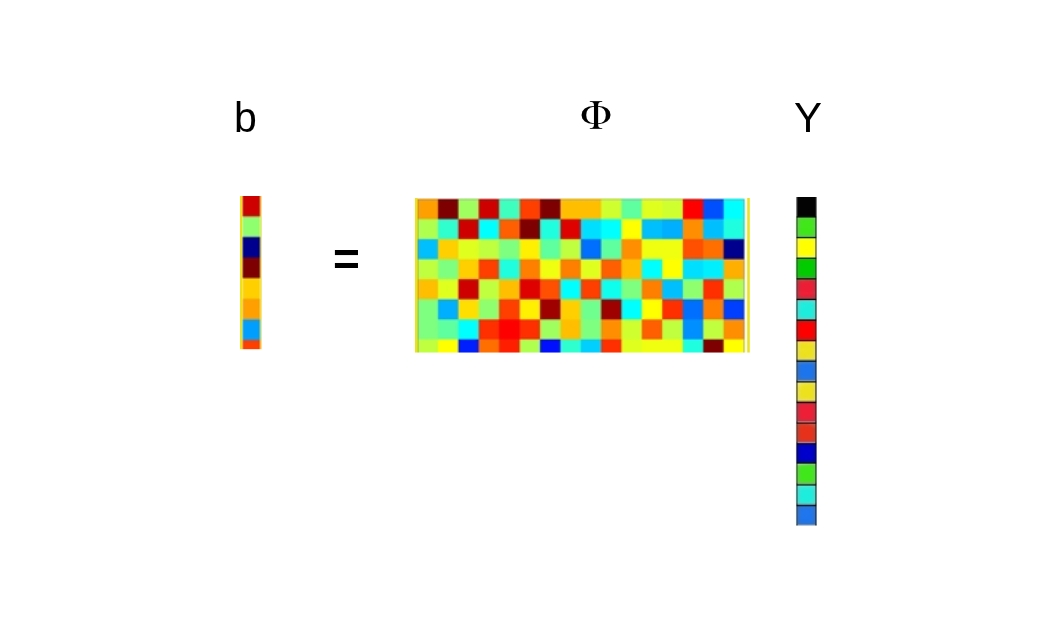
\includegraphics[height = 8cm, width=11cm]{figures/1}
    \caption{$ b= \Phi y$}
    \label{Figci1}
  \end{center}
\end{figure}

$\Phi$ is $M \times N$ matrix where $M<<N$.Now suppose we have $y= \Psi x$ where $x$ is a $k$-sparse representation of 
$y$ and $\Psi$ is the basis matrix. 
\newpage
\begin{figure}[!htbp]
  \begin{center}
      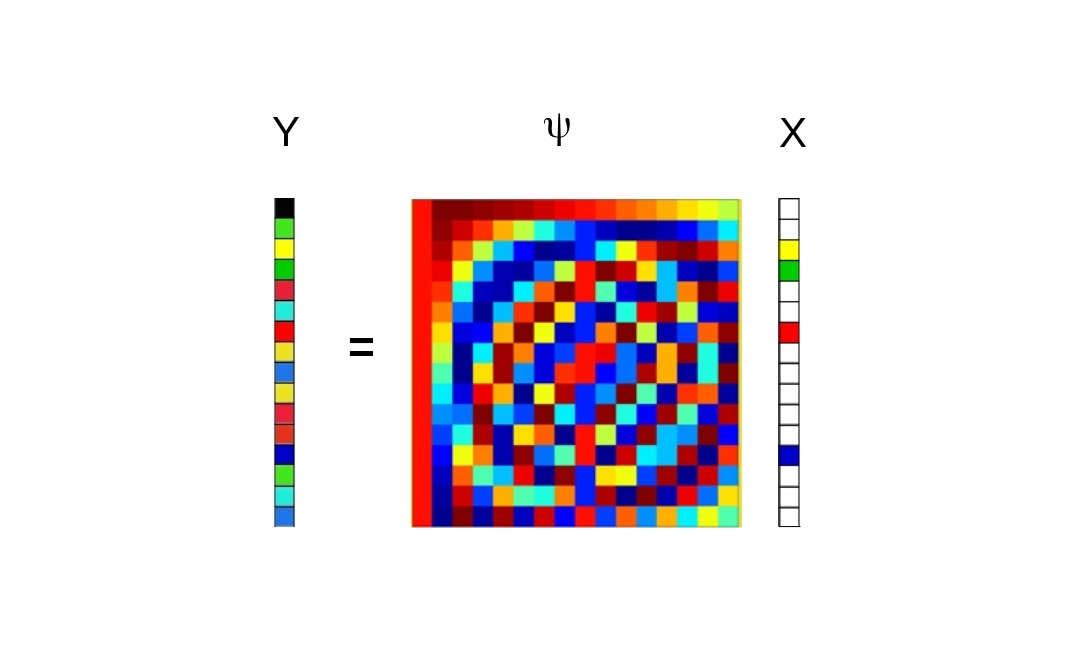
\includegraphics[height = 6cm, width=10cm]{figures/2}
    \caption{$ y = \Psi x$ }
    \label{Figci2}
  \end{center}
\end{figure}
The complete idea of compressed sensing is shown in following figure.

\begin{figure}[!htbp]
  \begin{center}
      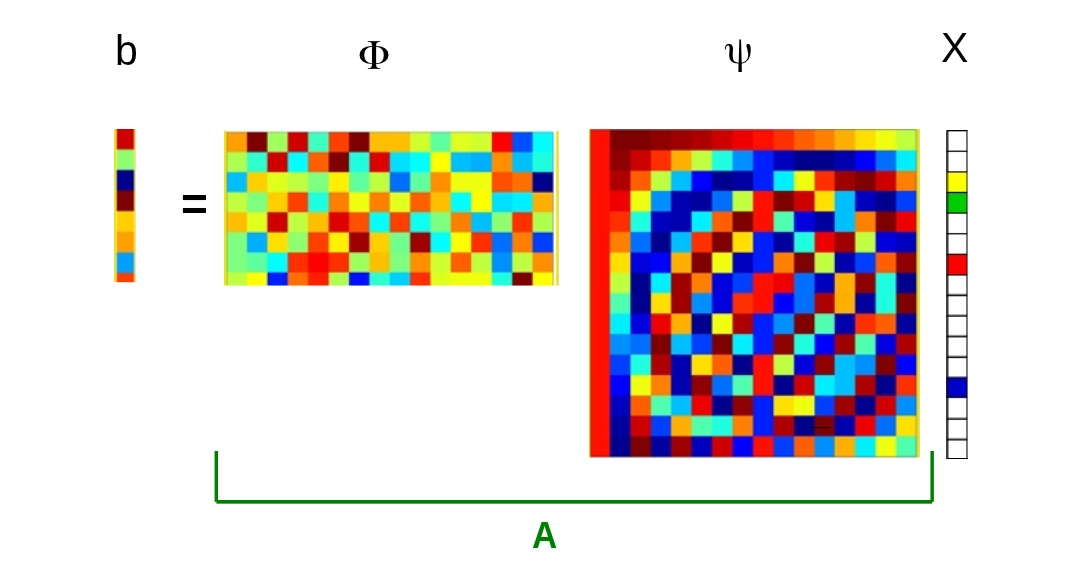
\includegraphics[height = 6cm, width=11cm]{figures/3}
    \label{Figci3}
  \end{center}
\end{figure}
In figure \ref{Figci3} equation $b = \Phi \Psi x$ is in $Ax = b$ form with $A = \Phi \Psi$.
Since $x$ is $k$-sparse, $x$ must be in one of the $C(n,k)$ subspaces of $R^N$. So if we have 
$m > k+1$ then exhaustive search can be done through these subspaces and we can determine which subspace $y$ belongs to.
This can be formulated as an optimization problem 

\begin{equation}
\mbox{minimize} \parallel x \parallel_{\ell_0} \mbox{subjected to }Ax=b
\label{1.2.1}
\end{equation}
where $\ell_0$ is the quasi-norm and is defined as 
\begin{equation}
 \parallel x \parallel_{\ell_0} =\displaystyle\sum\limits_{i=1}^{i=n}  I(x_i \neq 0) 
\label{1.2.2}
\end{equation}

where $I$ is an indicator function defined as 
\begin{equation}
I(x) =\left\lbrace
\begin{array}{lll}
  & 1 & x \neq 0\\
 & 0 & x = 0
\end{array}\right.
\label{1.2.3}
\end{equation}

\paragraph{}But performing this exhaustive search over all subspaces is computationally
intractable as $N$ increases (keeping $\alpha$ constant). One way of circumventing this problem is by using the $\ell_2$
norm as a proxy, which is equivalent to solving the following optimization problem. 

\begin{equation}
\mbox{minimize} \parallel x \parallel_{\ell_2} \mbox{subjected to }Ax=b
\label{1.5}
\end{equation}

\paragraph{}Solving the above equation leads to a solution for $Ax=b$ but it only guarantees $x$ to be small 
in the $\ell_2$ norm sense. In other words it does not help in reducing the number of non-zero components in the solution vector $x$ 
which is our prime aim.

%\begin{eqnarray}
%CIF: \hspace*{5mm}F_0^j(a) &=& \frac{1}{2\pi \iota} \oint_{\gamma} \frac{F_0^j(z)}{z - a} dz
%\end{eqnarray}
\nomenclature[zcif]{$CIF$}{Cauchy's Integral Formula}                                % first letter Z is for Acronyms 
\nomenclature[aF]{$F$}{complex function}                                                   % first letter A is for Roman symbols
\nomenclature[gp]{$\pi$}{ $\simeq 3.14\ldots$}                                             % first letter G is for Greek Symbols
\nomenclature[gi]{$\iota$}{unit imaginary number $\sqrt{-1}$}                      % first letter G is for Greek Symbols
\nomenclature[gg]{$\gamma$}{a simply closed curve on a complex plane}  % first letter G is for Greek Symbols
\nomenclature[xi]{$\oint_\gamma$}{integration around a curve $\gamma$} % first letter X is for Other Symbols
\nomenclature[rj]{$j$}{superscript index}                                                       % first letter R is for superscripts
\nomenclature[s0]{$0$}{subscript index}                                                        % first letter S is for subscripts

\paragraph{}Hence, minimizing the $\ell_0$-norm is computationally intractable and $\ell_2$-norm does not lead to sparse solutions.
A novel way of getting a sparse solution is by minimizing the $\ell_1$-norm subjected to $Ax = b$.

\begin{equation}
\mbox{minimize} \parallel x \parallel_{\ell_1} \mbox{subjected to }Ax=b
\label{1.6}
\end{equation}

\paragraph{}Solving this optimization problem leads to a sparse solution. It also guarantees the uniqueness in
solution as proved in .

\subsection{$\ell_1$ vs $\ell_2$}
\label{s:l1_vs_l2}

\paragraph{}One way of visualizing why $\ell_1$ leads to sparse solution and $\ell_2$ does not is shown in the 
following figure.

\begin{figure}[!htbp]
  \begin{center}
      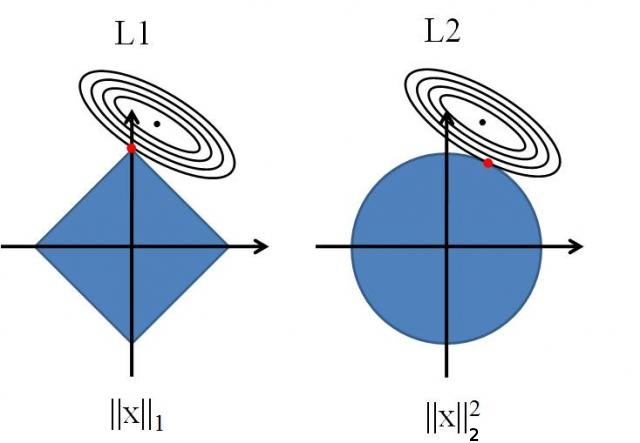
\includegraphics[height = 8cm, width=11cm]{figures/final_l1vsl2}
    \caption{$\ell_1$ vs $\ell_2$ ball}
    \label{Figl1vsl2}
  \end{center}
\end{figure}

\paragraph{}Figure (\ref{Figl1vsl2}) shows the $\ell_1$ ball and $\ell_2$ ball touching the contours of 
$\parallel Ax - b \parallel_{\ell_2}^2$. This clearly shows that due to the sharper corners of the $\ell_1$ ball,
contours of $\parallel Ax - b \parallel_{\ell_2}^2$ touch the $\ell_1$ ball at one of the axes, which is a sparse 
solution. However the $\ell_2$ ball is spherical and does not leads to a sparse solution.

\paragraph{}In general any $p$-norm is defined as 
\begin{equation}
 \parallel x \parallel_p = ( |x_1|^p + |x_2|^p + |x_3|^p +... |x_N|^p )^{\frac{1}{p}}
\label{1.7}
\end{equation}

\paragraph{}Further, an equivalent problem of minimizing the $p$-norm of $x$ is 
\begin{equation}
 minimize ( |x_1|^p + |x_2|^p + |x_3|^p +... |x_N|^p )
\label{1.8}
\end{equation}

\paragraph{}Let us compare the minimization of the $\ell_1$ norm and the $\ell_2$ norm. For the 
$\ell_2$ norm minimization, we care very little when $x_i < 1$ as compared to $\ell_1$ minimization because $\ell_2$ norm deteriorates
the smaller components more rapidly as compared to$ \ell_1$ norm. On the other hand 
during $\ell_2$ minimization we have a strong dislike when if $x_i > 1$. Hence, during minimization $\ell_2$
puts strong weights on larger components and a small weight (or zero weight) on smaller components of $x$ as
compared to the $\ell_1$ norm. So $\ell_1$ norm minimization places a larger emphasis on minimizing the smaller components
which in turn makes most of the components zero or approximately zero. This simple interpretation gives a clearer 
insight into why a solution of equation (\ref{1.6}) leads to sparse result. 

%Now I would like to cite the following: \cite{latex} and \cite{texbook}
%and \cite{Rud73}.

\subsection{Theorems for Compressed Sensing}
\label{s:cs_theorems}

\subsubsection{Restricted Isometry Property (RIP) or Uniform Uncertainty Principle (UUP)}

\paragraph{}UUP stands for “Uniform Uncertainty Principle“ (\cite{cand05}, \cite{cand07}). Matrices which follow these principle 
are called "UUP matrices". UUP matrices can compress vectors from high-dimensional space to low-dimensional space while
still being able to reconstruct these vectors. 

\paragraph{}In general, a $M \times N$ rectangular matrix $A$ is called orthogonal only if $M \geq N$ and each
column vector are orthonormal i.e. they all have unit length and are orthogonal to each other. Let 
$v_1, v_2 ... v_N$ be the '$N$' columns of $A$ matrix. Then
\begin{equation}
 v_i^*v_j   = 0 \hspace{10mm} \mbox{where } i \neq j \mbox{ and } i,j \mbox{ is from } 1 ... N
\label{1.9}
\end{equation}
\begin{equation}
 \parallel v_i \parallel_{\ell_2} = 1 \hspace{10mm} \mbox{where } i \mbox{ is from } 1 ... N
\label{1.10}
\end{equation}

\paragraph{}So this $A$ matrix can transform an $N$-dimensional vector $a =(a_1, a_2 ...a_N)$ to corresponding $M$ dimensional
vector, which is $ \displaystyle\sum\limits_{j=1}^{j=N} a_j v_j$. Now if this $A$ matrix is orthogonal, we know that norm 
of vectors are not changed when they are linearly transformed by an orthogonal matrix. So for above situation, we have
\begin{equation}
 \parallel \displaystyle\sum\limits_{j=1}^{j=N} a_j v_j \parallel_{\ell_2}^2  = \displaystyle\sum\limits_{j=1}^{j=N} |a_j|^2
\label{1.11}
\end{equation}

\paragraph{}This implies that $(a_1, a_2, ... a_N) \mapsto \displaystyle\sum\limits_{j=1}^{j=N} a_j v_j $ is an isometry i.e. 
given the encoded vector $ z = \displaystyle\sum\limits_{j=1}^{j=N} a_j v_j$ one can uniquely recover the original coefficients 
$(a_1, a_2 ... a_N)$. Furthermore, small changes in $z$ will not cause large fluctuations in $(a_1, a_2 ... a_n)$. Indeed, 
one can reconstruct the original coefficients quickly and explicitly by the formula 
\begin{equation}
 a_j = < z, v_j> 
\label{1.12}
\end{equation}

\paragraph{}But in the Compressed Sensing setting we cannot apply this property directly as we have $M << N$. In other words we 
cannot express a vector of say in '$t$' dimension with a basis vectors set of cardinality greater than $t$. So for our case

\begin{equation}
 a_1 v_1 + a_2 v_2 + ... +a_n v_N =0
\label{1.13}
\end{equation}
 
\paragraph{}If we can try to overcome the above restriction by weakening equation (\ref{1.11}) for all $(a_1,a_2, ... a_n)$ by
\begin{equation}
  (1-\delta_1)\displaystyle\sum\limits_{j=1}^{j=n} |a_j|^2 \hspace{3mm} \leq \hspace{3mm} \parallel \displaystyle\sum\limits_{j=1}^{j=n} a_j v_j \parallel_{\ell_2}^2  \hspace{3mm} \leq \hspace{3mm} (1+ \delta_2)\displaystyle\sum\limits_{j=1}^{j=n} |a_j|^2
\label{1.14}
\end{equation}
\paragraph{}where $\delta_1,\delta_2$ are constants such that $0 < \delta_1 \delta_2< 1 $. The above condition is as good
as saying columns of the matrix are locally orthogonal rather than globally perfectly orthogonal. Due to this property 
which is also called as \emph{Restricted Isometry Property (\cite{cand05, cand07})}, it turns out that one can pack more 
than $M$ vectors into $M$ dimensional space if one localizes the almost orthogonality condition so that it only holds for sparse sets of coefficients $(a_1,a_2, ... a_N)$. 
Sparsity parameter $k$ (less than $M$) plays an important role here. If we say that our sensing matrix $A$ obeys the UUP 
with sparsity $k$ then one has the almost orthogonality condition (\ref{1.14}) for any set of coefficients $(a_1,a_2, ... a_N)$, 
such that at most $k$ of the $a_j$ are non-zero. In other words, we only assume that any $k$ of the $N$ vectors $v_1, v_2,... v_N$
are almost orthogonal at one time. 

\paragraph{}Furthermore, constructing UUP matrices is an NP hard problem. In other words there is no polynomial 
time algorithm known which can construct these UUP matrices. The best possible methods are the one which could simply
search through all matrices in a given class and test each one of them for the UUP property. But this is an exponential-time
algorithm. However it has also seen that some matrices like random normalized Gaussian matrices, random normalized Bernoulli matrices are
UUP matrices. But they are all probabilistic in nature; in particular, these constructions are not 100\% guaranteed to actually produce
a UUP matrix, although in many cases the failure rate can be proven to be exponentially small in the size of the matrix. 
So for many larger scale applications it is actually exponentially less prone to failure.

\newtheorem*{mydefo}{Definition}
\begin{mydefo}
UUP matrices are the generalization of (rectangular) orthogonal matrices in which columns are locally 
almost orthogonal rather than globally perfectly orthogonal.
\end{mydefo}

\subsubsection{Incoherence}

\paragraph{}In Compressed Sensing we are dealing with two matrices $\Phi$ (sensing Matrix)
and $\Psi$ (Basis matrix which is used to represent $y$ in sparse basis). Coherence between the sensing
basis and Basis matrix defined as 
\begin{equation}
\mu(\Phi,\Psi) = \sqrt{N} max_{1\leq k, j\leq N} |<\Psi_k,\Phi_j>|
\end{equation}
\paragraph{}In simple words, coherence($\mu$) measures the largest correlation between two elements of $\Phi$ and $\Psi$. If
$\Phi$ and $\Psi$ contain correlated elements, then the coherence is large. Compressed Sensing is mainly concerned with
low coherence pairs i.e. we require low values of $\mu$. Classical example of incoherent basis pairs are the Fourier basis 
and Euclidean basis. These basis pairs are maximally incoherent with incoherence $\mu = 1$. Another example is pair of 
wavelets bases ($\Psi$) and noiselets $(\Phi$). The coherence between noiselets and Haar wavelets is $\sqrt{2}$ and 
between noiselets and Daubechies D4 and D8 wavelets, respectively, about 2.2 and 2.9. Noiselets are also maximally incoherent
 with euclidean basis and Fourier basis.

\paragraph{}Finally, random matrices are largely incoherent with any fixed basis $\Psi$. We select an orthobasis $\Psi$ 
uniformly at random, which can be done by orthonormalizing $N$ vectors sampled independently and uniformly on the unit 
sphere. Then with high probability, the coherence between $\Psi$ (Basis Matrix) and $\Phi$ (Sensing basis matrix) is 
$\simeq$ $\sqrt{2 logN}$. Random Gaussian i.i.d matrices also show very low coherence with fixed representation basis matrix $\Psi$.


\newtheorem{csth}{THEOREM (\cite{cand07})}
\begin{csth}
 Suppose $y \in R^N$ is sparse in some $\Psi$ basis and $x \in R^N$ is $k$-sparse representation of $y$. Now we select
$M$ measurements in $\Phi$ uniformly at random. Then if 
\begin{equation}
 M \geq C \mu^2(\Phi,\Psi)klogN
\end{equation}
for some constant $C$ the solution \ref{1.6} is exact with overwhelming probability.
\end{csth}

\paragraph{}The role of coherence is now clear; the smaller the coherence, the fewer samples are needed,
hence compressed sensing require low coherence pairs of basis matrices. One suffers no information loss by measuring just
about any set of $M$ coefficients which may be far less what the signal size apparently demands. If $\mu(\Phi,\Psi)$ is equal or
close to one, then of the order of $klogN$ samples suffice instead of $N$.

\subsection{Applications}
\label{s:cs_applications}
The fact that sparse signals can be reconstructed efficiently using very few number of incoherent
samples which is proportional to sparsity ($k$) has far reaching implications and applications. The main 
areas where compressed sensing had proven itself as a more advantageous and efficient technique are
\begin{itemize}
 \item \emph{Data compression}. In some situations, the sparse basis $\Psi$ may be unknown at the encoder or impractical to implement
for data compression. However a randomly designed $\Phi$ can be considered a universal encoding strategy, as it need not be 
designed with regards to the structure of $\Psi$. This universality may be particularly helpful for distributed source
coding in multi-signal settings such as sensor networks (\cite{baron09}).
 \item Channel coding. Compressed Sensing principles can be turned around and applied to design fast error correcting codes over
the reals to protect from errors during transmission (\cite{cand05}).

 \item \emph{Inverse problems}. The only way to acquire $x$ may be to use a measurement system $\Phi$ of a certain
    modality. However, assuming a sparse basis $\Psi$ exists for $x$ that is also incoherent with $\Phi$, then efficient sensing will
    be possible. One such application involves MR angiography and other types of MR setups, where $\Phi$ records a
    subset of the Fourier transform, and the desired image $x$ is sparse in the time or wavelet domains (\cite{lustig06}).

 \item \emph{Data acquisition}. Finally, in some important situations the full collection of $N$ discrete-time samples of an analog signal
may be difficult to obtain (and possibly difficult to subsequently compress). Here, it could be helpful to design physical
sampling devices that directly record discrete, low-rate incoherent measurements of the incident analog signal.

\end{itemize}

\section{Radio Interferometry}
\label{s:radio_astronomy}

\subsection{Radio Telescopes and its Resolution}
\label{s:radio_telescope}

\paragraph{}Angular resolution ($\theta$) of a telescope depends on the wavelength of light or 
radio waves ($\lambda$) and the diameter (D) of the telescope being used.
The relation between $\theta$, $\lambda$ and $D$ is given by
\begin{equation}
 \theta \sim  \lambda/D
\label{2.1}
\end{equation}
Here $\theta$ is in radians and $\lambda$ and $D$  in meters.

\paragraph{}Radio telescopes are used to study radio waves emitted by astronomical objects
of wavelengths roughly between about 10 meters and 1 millimeter. It is possible to 
observe radio waves from the ground as shown in the figure \ref{Fignasa}, spacecraft are needed to
observe astronomical objects in gamma rays, X-rays, UV, and IR, while ground observations 
are possible in the visible, some parts of the near IR, and the radio.
\begin{figure}[!htbp]
  \begin{center}
      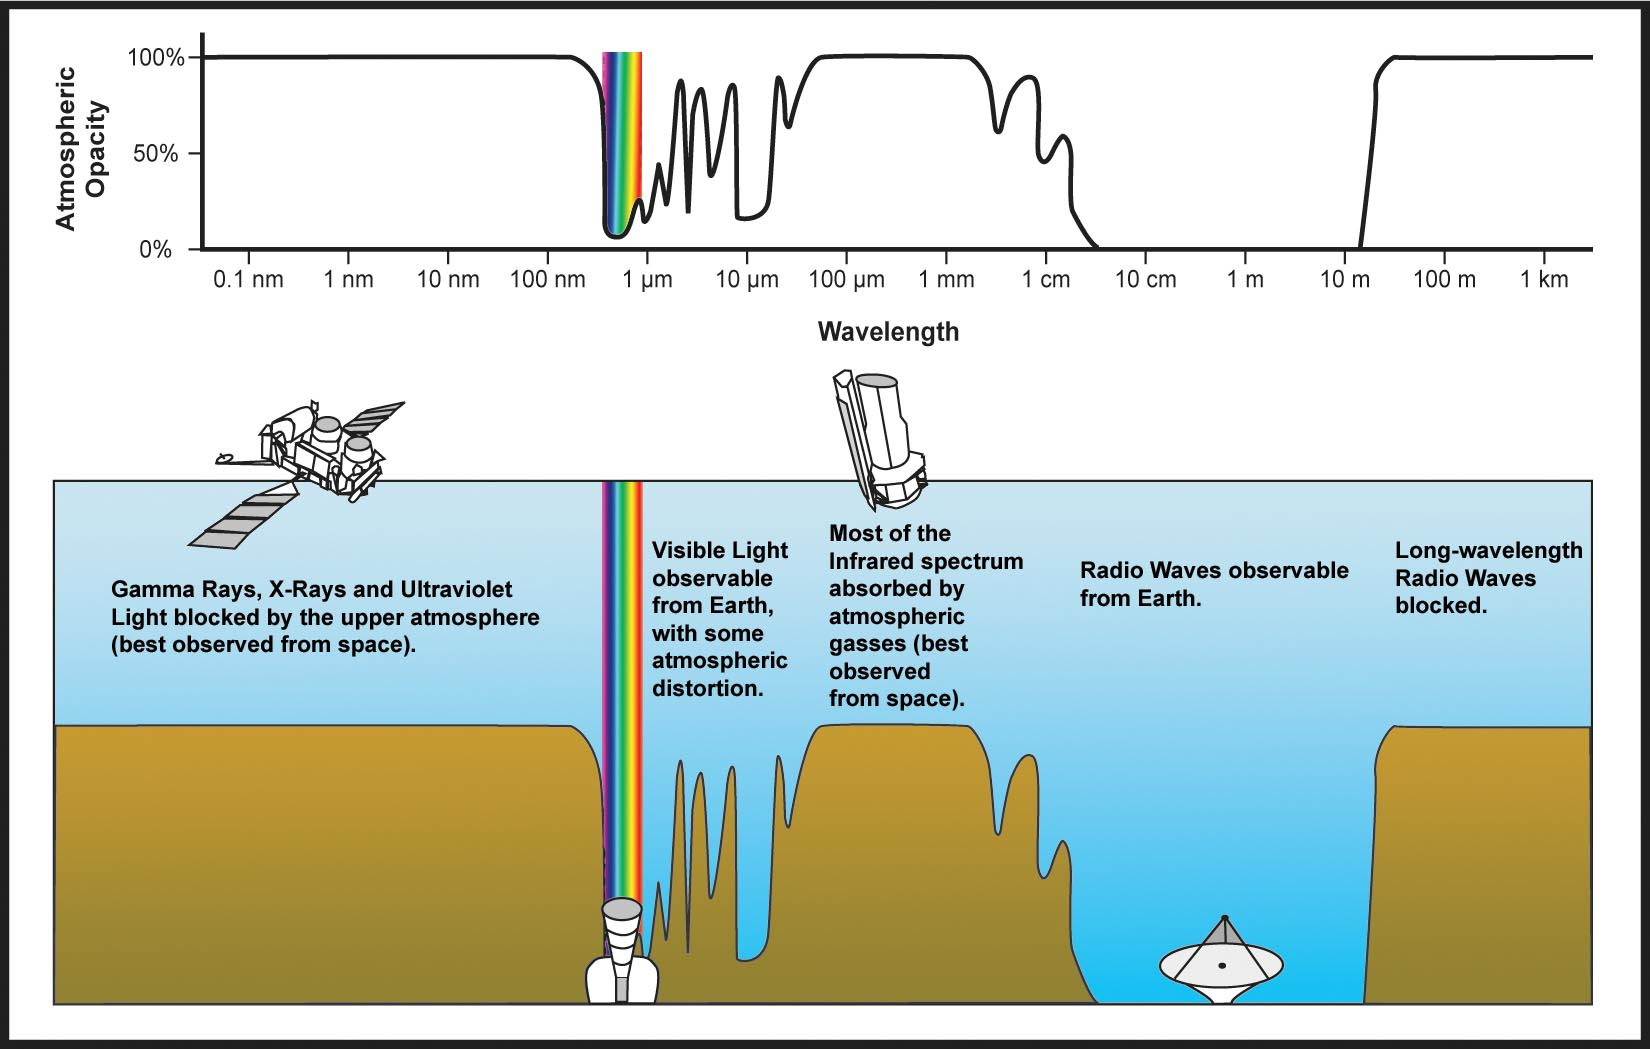
\includegraphics[width=6.1in,height=4in]{figures/nasa}
    \caption{Image credit : NASA/IPAC}
    \label{Fignasa}
  \end{center}
\end{figure}

\paragraph{}Due to larger operating wavelengths and primarily because of relation equation (\ref{2.1}), 
radio telescopes have to be much larger than optical telescopes to attain good angular resolution. Angular resolution 
is a measure of how small detail of an area in the sky can be seen. The larger the telescope, the more 
detail can be observed in a given wavelength.

\subsection{Radio Interferometry}
\label{s:radio_interferometry}

\paragraph{}Angular resolution of telescope given by equation (\ref{2.1}) is limited by its operating wavelength and 
diameter of aperture. To get good resolution, one has to either decrease the operating wavelength or 
increase the size of telescope. In radio astronomy, the wavelengths are so large that even though the 
sizes of radio telescopes are large, the angular resolution is poor as compared to optical instruments.
With these larger telescopes one can achieve higher resolutions by operating wavelengths in the
centimeter to millimeter range. Telescopes of hundreds of meters in diameter are needed to observe the source 
at metre wavelengths which would clearly impractical.

\paragraph{}Radio astronomers achieve higher resolution at metre wavelengths using a technique called 
\emph{Radio Interferometry}. The interferometers like GMRT (\cite{gmrt}) consist of array of antennas 
located on ground and resolution of such a telescope is proportional to maximum projected distance 
between the antennas. The separations between antennas are called as \emph{Baseline} and are measured in units of wavelength
($\lambda$). 

\subsubsection{Van Cittert \textendash Zernike theorem}

\paragraph{}Van Cittert \textendash Zernike theorem is the key theorem in radio interferometric imaging.
 It relates the spatial coherence function at two points on the ground also called Visibility function ($V(r_1,r_2)$)
 with the distribution of source intensity $I$. It also shows that the visibility function $V(r_1,r_2)$ depends only on the 
relative distances between two points i.e $r_1-r_2$

\paragraph{}As explained in \cite{ncrabookchap2}. Let us consider a two element interferometer with antenna 1 and antenna 2 
located on ground at $P_1(x_1,y_1,z_1)$ and $P_2(x_2,y_2,z_2)$ respectively. 
Consider an infinitesimal element of the source positioned at $P(x,y,z)$ in the sky shown in figure ().
If electric field intensity at the point $P$ is given by $\varepsilon(P)$, then the electric field at
the observation point $P_1$ \cite{wolf} is given by
\begin{equation}
 E(P_1) = \int \varepsilon(P) \frac{e^{-\frac{2\pi}{\lambda}D(P_1,P)}} {D(P_1,P)}d\Omega
\label{2.2}
\end{equation}
\paragraph{}where $D(P_1,P)$ is defined as the distance between the points $P$ and $P_1$. $\Omega$ is the solid 
angle subtend by the infinitesimal source at $P$.Assuming that the emission from the source is spatially incoherent,
at point $P_2$ the electric field is given by
\begin{equation}
 E(P_2) = \int \varepsilon(P) \frac{e^{-\frac{2\pi}{\lambda}D(P_2,P)}} {D(P_2,P)}d\Omega
\label{2.3}
\end{equation}

The spatial coherence function is given by
\begin{equation}
 < E(P_1)E^*(P_2)> = \int <\varepsilon(P)\varepsilon^*(P)> \frac{e^{-\frac{2\pi}{\lambda}(D(P_2,P)-D(P_2,P))}} {D(P_1,P) D(P_2,P)}d\Omega
\label{2.4}
\end{equation}

where Intensity($I$) of the source is defined as 
\begin{equation}
 I(P)=<\varepsilon(P)\varepsilon^*(P)>
\label{2.5}
\end{equation}

If we imagine a celestial sphere of radius $R$ and approximate the source lying on this sphere then we have $x=R cos(\theta_x)$
$y=R cos(\theta_y)$ and $z=R cos(\theta_z)$ where $cos(\theta_x),cos(\theta_y),cos(\theta_z)$ are direction cosine $l,m,n$.
Also $l^2+m^2+n^2=1$ and the solid angle $\Omega = \frac{dldm}{\sqrt{1-l^2-m^2}}$. Further \\\\
$
\begin{array}{rl}
  D(P_1,P) = &  [ (x-x_1)^2 + (y-y_1)^2 + (z-z_1)^2]^{\frac{1}{2}}\\
           = &  [ (Rl-x_1)^2 + (Rm-y_1)^2 + (Rn-z_1)^2 ]^{\frac{1}{2}}\\
	   = &  R[(l-x_1/R)^2 + (m-y_1/R)^2 + (n-z_1/R)^2 ]^{\frac{1}{2}}\\
	   \simeq & R [(l^2+m^2+n^2)-2/R(lx_1+my_1+nz_1)]^{\frac{1}{2}}\\
	   \simeq & R-(lx_1+my_1+nz_1)
\label{hello}
\end{array}
$\\
Similarly we have 
\begin{equation}
 D(P_2,P) = R-(lx_2+my_2+\sqrt{1-l^2-m^2}z_2)
\label{2.6}
\end{equation}
Using above equations we can approximate $D(P_1,P) D(P_2,P)$ as $R^2$ as shown below\\\\
$
\begin{array}{rl}
  D(P_1,P)D(P_2,P) =& \{R-(lx_1+my_1+nz_1)\}\{R-(lx_2+my_2+nz_2)\}\\
		   =& R(R-(l(x_1+x_2)+m(y_1+y_2)+z(z_1+z_2)) \\&+ (lx_2+my_2+nz_2)(lx_1+my_1+nz_1)
\end{array}
$\\\\
In above equation $R-(l(x_1+x_2)+m(y_1+y_2)+z(z_1+z_2) \simeq R$ and further \\$R^2>>(lx_2+my_2+nz_2)(lx_1+my_1+nz_1)$.
Hence we have 
\begin{equation}
 D(P_1,P)D(P_2,P) \simeq R^2
\label{2.7}
\end{equation}

Putting the above equations (\ref{2.5}),(\ref{2.7}) in equation (\ref{2.4}) we have
\begin{equation}
 < E(P_1)E^*(P_2)> = \frac{1}{R^2}\int I(P) e^{-\frac{2\pi}{\lambda}(l(x_2-x_1)+m(y_2-y_1)+n(z_2-z1))} \frac{dldm}{\sqrt{1-l^2-m^2}}
\label{2.8}
\end{equation}

Above equation () is the full Van Cittert-Zernike equation. It can be seen from above equation spatial coherence function or
visibility function $V(r_1,r_2)=< E(P_1)E^*(P_2)>$ depends upon $r_1-r_2$. We define baseline co-ordinates $u,v,w$ such that 
$u = (x_2-x_1)/\lambda$, $v = (y_2-y_1)/\lambda$ and $w = (z_2-z_1)/\lambda$ and also since we have relation $l^2+m^2+n^2=1$
the above equation reduced to
\begin{equation}
V(u,v,w) = \frac{1}{R^2}\int I(l,m) e^{-\frac{2\pi}{\lambda}(lu+mv+(\sqrt{1-l^2-m^2})w)} \frac{dldm}{\sqrt{1-l^2-m^2}} 
\label{2.9}
\end{equation}

\subsubsection{Two-Dimensional Approximation}

Equation (\ref{2.9}) under certain assumption can be approximated as two-dimensional Fourier transform of the source intensity
distribution. If we confined our observation to $u-v$ plane i.e when $w=0$ then we have 
\begin{equation}
V(u,v) = \frac{1}{R^2}\int I(l,m) e^{-\frac{2\pi}{\lambda}(ul+vm)} \frac{dldm}{\sqrt{1-l^2-m^2}} 
\label{2.10}
\end{equation}
Another approximation to above equation is when we consider that the source brightness distribution is limited only
to small region of sky. In this case $n =\sqrt{1-l^2-m^2} \simeq 1$. Then the equation (\ref{2.9}) becomes

\begin{equation}
V(u,v) = \frac{1}{R^2}\int I(l,m) e^{-\frac{2\pi}{\lambda}(ul+vm)} dldm
\label{2.11}
\end{equation}
Source brightness is described in $lm$ plane while the equivalent conjugate variables in Fourier space $u,v$ is
described in $uv$ plane.$u,v$ is interpreted as spatial frequency and Visibility function $V(u,v)$ as spatial
frequency spectrum of source brightness distribution. 


\subsection{Dirty Beam and Dirty Image}
\label{s:radio_dirty}

Fourier transform relation exists between source brightness $I$ and the visibility $V$ we can take 
an inverse Fourier transform which can be given by
\begin{equation}
 I(l,m) = \int_{-\infty}^{+\infty}\int_{-\infty}^{+\infty} V(u,v) e^{2\pi i (ul+vm)} dudv
\label{2.12}
\end{equation}
Since it is impractical to cover whole $uv$ plane, we measure visibilities only at some points. Due to which image of sky
is not the true image but comes with lot of noise such an image is called Dirty Image is given by 
\begin{equation}
 I^D(l,m) = \int_{-\infty}^{+\infty}\int_{-\infty}^{+\infty} S(u,v) V(u,v) e^{2\pi i (ul+vm)} dudv
\label{2.13}
\end{equation}
where $V(u,v)$ is observed visibility and $S(u,v)$ denote sampling function which is indicator of where
on $u-v$ plane visibilities are measured. It is given by 

\begin{equation}
S(u,v) = \delta(u-u_k,v-v_k)
\label{2.14}
\end{equation}

Hence practically we measure sampled Visibility function ($V^S(u,v)$) which is given by
\begin{equation}
V^S(u,v) = \delta(u-u_k,v-v_k)V(u_k,v_k)
\label{2.15} 
\end{equation}
 where $(u_k,v_k)$ are the co-ordinates of points where visibility is measured. Hence
the discretized form of visibility function with discretized $l-m$ grid with reference to equation (\ref{2.11}) is
given by
\begin{equation}
 V(u_j,v_j)= \displaystyle\sum\limits_{k=1}^{k=N} I(l_k,m_k) e^{2\pi i (u_jl_k+v_jm_k)}
 \label{extra}
\end{equation}
Note above equation denotes only one visibility at $(u_j,v_j)$.\\
In short we have $V^S = SV$. If $F$ denote Fourier operator then equation (\ref{2.13}) can be written as,
\begin{equation}
 I^D = FV^S = F(SV)
\label{2.16}
\end{equation}
By Convolution theorem (\cite{bracewell}),
\begin{equation}
 I^D = FS * FV
\label{2.17}
\end{equation}
For a point source of unit strength at $(l_0,m_0)$, $|V(u,v)=1|$\\
$FV= \delta(l-l_0,m-m_0)$\\
$I^D = FS * FV = FS * \delta =  FS$. \\This is called the Dirty Beam which is given by
\begin{equation}
 B =FS
\label{2.18}
\end{equation}
Hence putting equation (\ref{2.18}) in equation (\ref{2.17}). Dirty Image is defined as the 
convolution of dirty beam and true image ($FV$).
\begin{equation}
 I^D = B * FV
\label{2.19}
\end{equation}

\subsection{Deconvolution}
\label{s:radio_deconvolve}

\paragraph{}The deconvolution problem in equation (\ref{2.19}) corrects for the $u-v$
plane sampling effect. The lack of measurement at certain interferometric spacing means 
that in principle an infinite number of brightness distributions could be consistent with
our visibility data. On the other hand, we may incorporate additional information to constrain
our solutions. The most widely used deconvolution method are CLEAN (\cite{hogbom}) and Maximum
Entropy Minimization

\subsubsection{CLEAN Algorithm}
CLEAN algorithm consider sky as containing only isolated point sources and approximates an image by a collection of point sources.
It then deconvolve each point source using a simple iterative approach. The final deconvolved image which is also called CLEAN image 
is the sum of these CLEAN components convolved with a Gaussian beam. This algorithm was published by \cite{hogbom} in 1974 and several 
variations have been proposed since then. Following are the main steps of the CLEAN algorithm.
\begin{itemize}
 \item Find the peak in Dirty Image.
 \item Subtract a dirty beam ($B$) of approximate strength to remove its side-lobes.
 \item Construct CLEAN image $I'$ using position and magnitude of subtracted components.
 \item Continue looping until some threshold level is met.
 \item Convolve the final $I'$ with an idealized CLEAN beam.
\end{itemize}

\subsubsection{Maximum Entropy Minimization}

MEM method minimizes a smoothness function ("entropy") in an image.
Maximum entropy is also called the all-poles model or auto-regressive model.
For images with more than a million pixels, this algorithm is faster than CLEAN 
algorithm. Details of the algorithm can be found in \cite{}.

\subsection{GMRT}
\label{s:radio_gmrt}

\href{http://ncra.tifr.res.in}{National Centre for Radio Astrophysics ( NCRA )} has set up an international facility for radio astronomical research
in the metre wavelengths range of the radio spectrum known as the \href{http://gmrt.ncra.tifr.res.in}{Giant Metre wave Radio Telescope (GMRT)}. This is the
world's largest array of radio telescopes at metre wavelengths and is located at a site about 80 km north of Pune. 
GMRT consists of 30 fully steerable gigantic parabolic dishes of 45m diameter each spread over distances of upto 25 km.
There are fourteen telescopes randomly arranged in the central square 1 km by 1 km in size, with a further sixteen arranged
in three arms of a nearly "Y"-shaped array each having a length of 14 km from the array centre.

\begin{figure}[!htbp]
  \begin{center}
      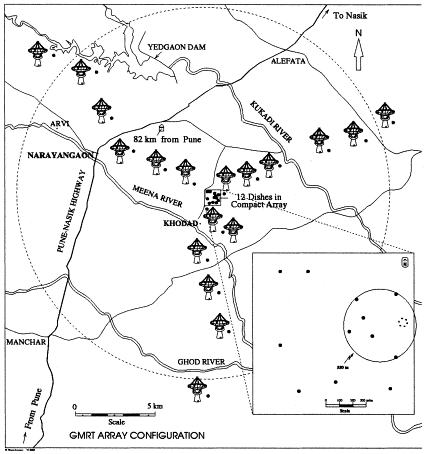
\includegraphics[height=6in]{figures/yshape}
    \caption{"Y" shaped Array}
    \label{FigYshape}
  \end{center}
\end{figure}

Antenna feeds at five different frequency centered at 153, 233, 327, 610, and 1420 MHz, with polarization. 
The maximum baseline in the array gives the telescope an angular resolution 
(the smallest angular scale that can be distinguished) of about 1 arc-second at the frequency of 1420 MHz.


\subsection{Compressed Sensing formulation for Radio Interferometry}
\label{s:radio_cs}
\paragraph{}Equation (\ref{2.11}) shows that under certain approximation, Visibility function is the Fourier transform of
source brightness. Radio Interferometers like GMRT measures visibility at very few points on $u-v$ plane.
At a time GMRT measures 435($C(30,2)$) visibilities. Each pair of antenna measures one visibility. This is 
shown in figure\footnote{Image by A.\ Basu, NCRA}(\ref{Figattime}) where each point represent one visibility.
\begin{figure}[!htbp]
 \hspace*{-10em}
 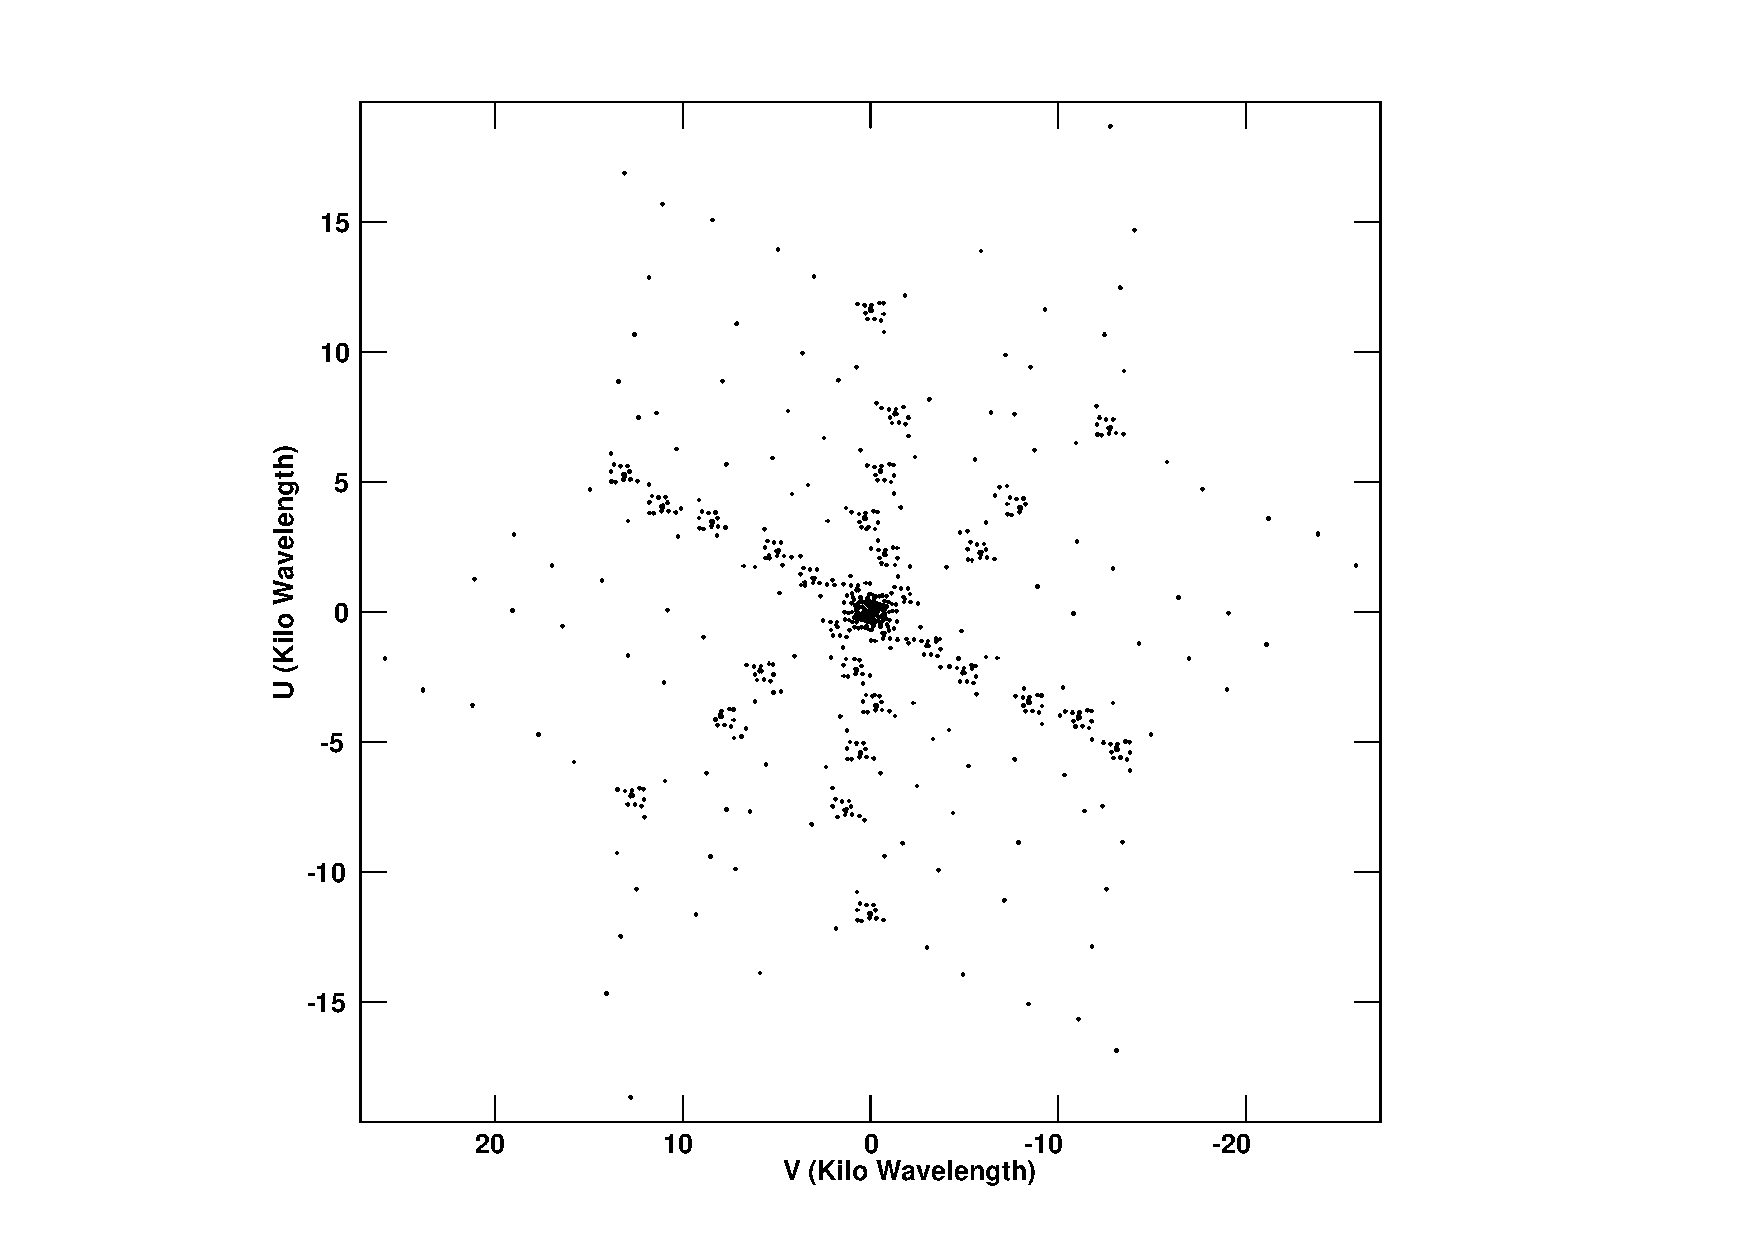
\includegraphics[width=1.5\textwidth]{figures/attime}
 \caption{$uv$ coverage at a time}
 \label{Figattime}
\end{figure}

% ------------------------------------------------------------------------
\begin{figure}[!htbp]
 \hspace*{-10em}
 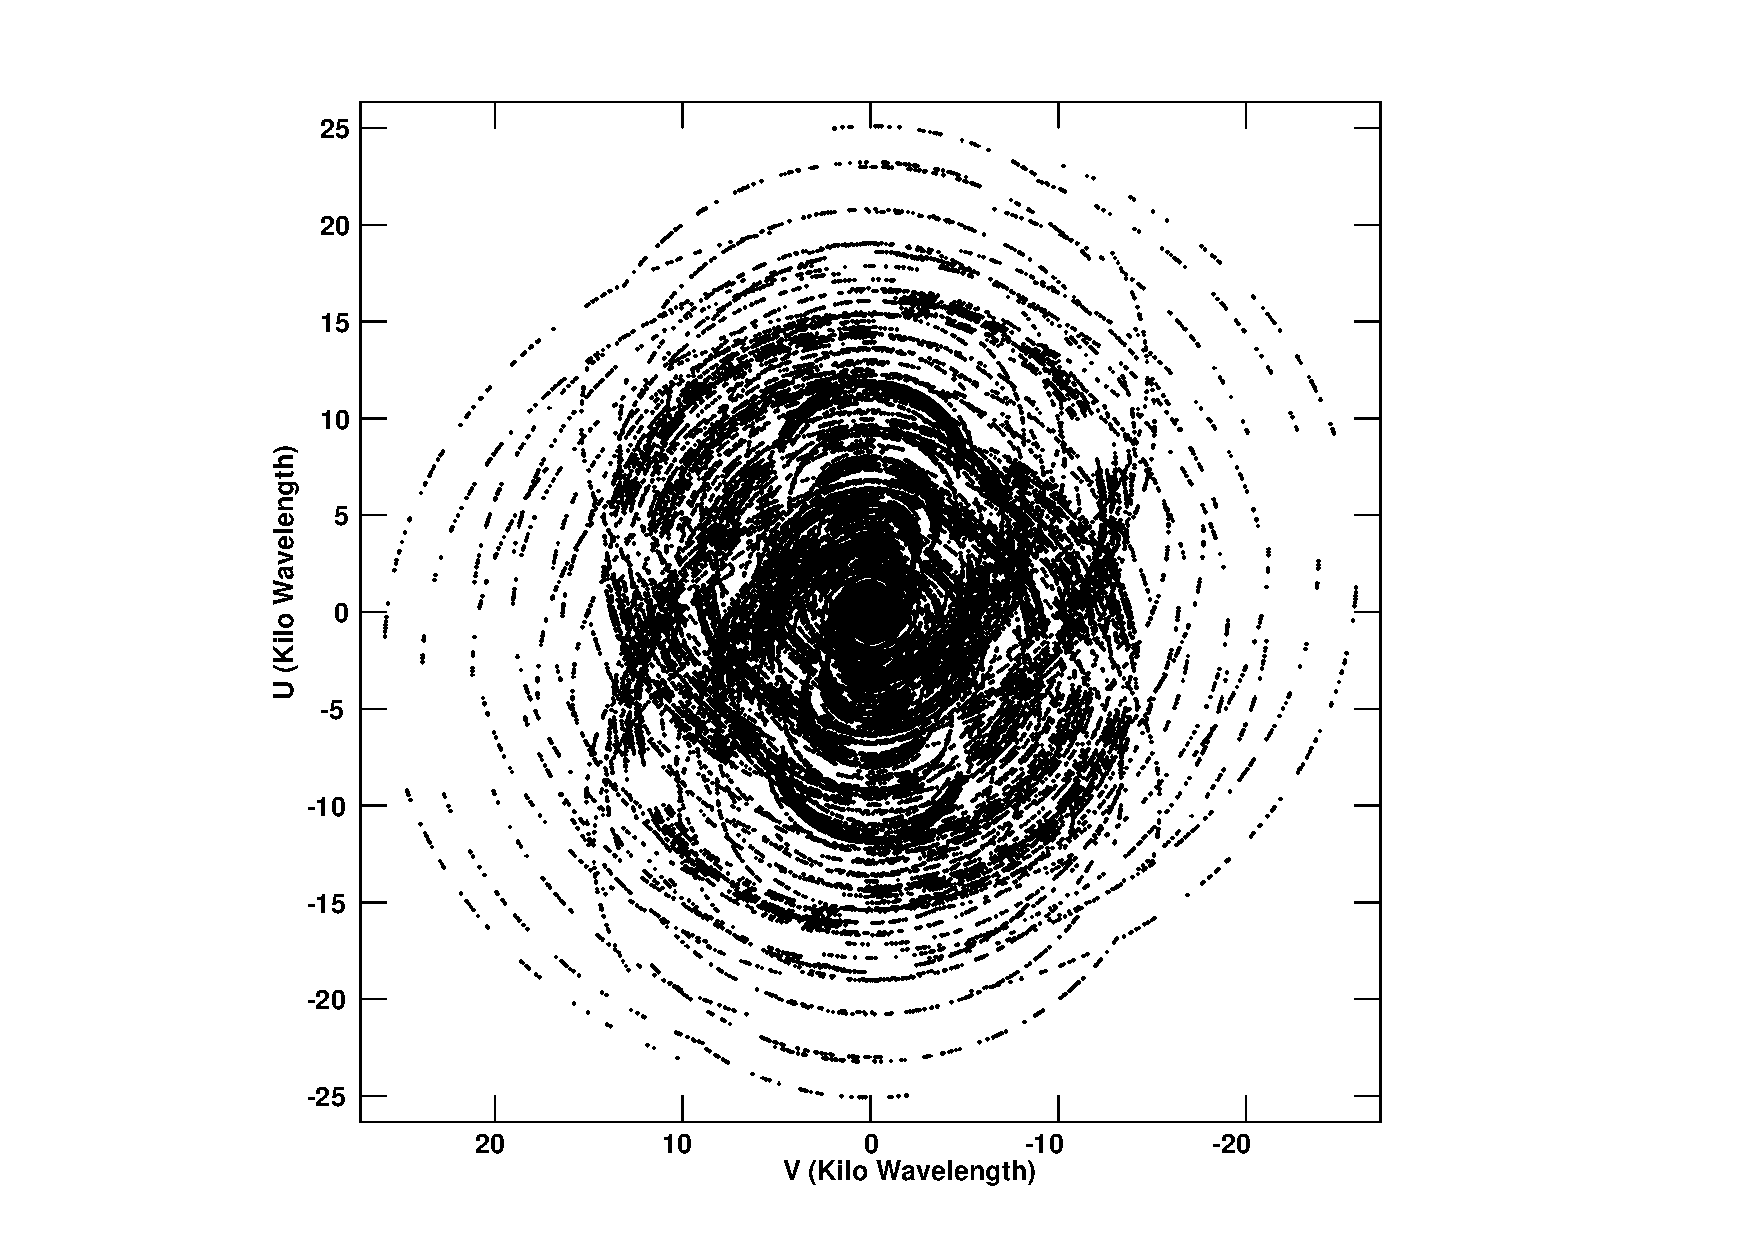
\includegraphics[width=1.5\textwidth]{figures/fewhrs}
 \caption{$uv$ coverage for few hours}
 \label{Figfewhrs}
\end{figure}
\newpage
\paragraph{}Due to rotation of earth, the projected separation between the antenna change and over certain time
it covers more point on the $u-v$ plane. This is shown in figure \footnote{Image by A.\ Basu, NCRA}(\ref{Figfewhrs})

\paragraph{}Even after few hours of $uv$ coverage (figure :\ref{Figfewhrs}) $uv$ coverage is not uniform.
Clearly we have under-sampled visibility data and hence Compressed Sensing methods proven to be viable option. Equation (\ref{2.11})
can be cast in to compressed sensing setting with visibilities as measurement vector and partial 2-D Fourier matrix as
measurement matrix and sky image as the unknown. In radio astronomy, most of the sources are point source so, most of the time
image is sparse in euclidean image. However there are the cases in which we have to represent image in some sparse basis which
can be done with some extra effort as in case of other application of compressed sensing.

\subsection{Why Compressed Sensing in Radio Astronomy?}
\label{s:radio_cs_why}
\paragraph{}In general, Compressed Sensing is advantageous when signals are sparse in some known basis, measurements are expensive and 
computations are cheaper at receiving end. These situations make Compressed Sensing methods a strong candidate for image 
deconvolution problem in radio astronomy. 
\paragraph{}Compressed Sensing methods can directly reconstruct the image from the sparse observations, without the need 
for an iterative deconvolution. Also it will be very efficient technique, when the 2-D approximation to Van Cittert-Zernike Theorem
breaks. Further with the advent of recent efficient and robust $\ell_1$ based algorithms, Compressed Sensing
takeover mainstream deconvolution methods used in Radio Astronomy like CLEAN and Maximum Entropy minimization as discussed 
in section 2.4. 










% ------------------------------------------------------------------------

%%% Local Variables: 
%%% mode: latex
%%% TeX-master: "../thesis"
%%% End: 

 % introduction
 \chapter{Algorithms for Compressed Sensing}
\label{c:algorithms}

\section{Algorithms}
\label{s:algorithms}

\paragraph{}Convex Optimization is a sub field of Optimization which can produce reliable solutions
and can be solved exactly. Many signal processing problems can be formulated as convex 
optimization problems of form
\begin{equation}
 minimize_{x \in R^N} \hspace{4mm}f_1(x) +f_2(x) + ... + f_{n-1}(x) +f_n(x)
\label{3.1}
\end{equation}

\paragraph{}where $f_1, f_2, ..., f_n$ are convex functions defined from $f:R^N$ $\rightarrow$ $R$ where some of the 
functions are non-differentiable, this which rules out our conventional smooth optimization
techniques like Steepest decent method, conjugate gradient method etc. We have explored
the class of algorithms which can solve equation (\ref{3.1}). These methods proceed by splitting, 
in that the functions $f_1, . . . , f_n$ are used individually so as to yield an easily
implementable algorithm. They are called proximal because each non smooth function in \ref{3.1} 
is involved via its proximity operator. Iterative thresholding, projected Landweber, projected
gradient, alternating projections, alternating-direction method of multipliers, alternating
split Bregman are special instances of proximal algorithms. Details of proximal methods are discussed in \cite{Com07}.

\subsubsection{Notations}
\paragraph{}Here after, $R^N$ is the $N$-dimensional euclidean space and domain of function 
$f: R^N  \rightarrow ]-\infty,+\infty]$. \\
\paragraph{}Let $C$ be the non-empty convex subset of $R^N$. The indicator function of $C$ is defined as

\begin{equation}
i_C : x \mapsto \left\lbrace \begin{array}{ll}
0        &  \mbox{if } x \in C\\
+ \infty & \mbox{if } x \notin C 
\end{array} \right.
\label{3.2}
\end{equation}

$p$-norm is defined as ( $\parallel . \parallel_{p}$ )
\begin{equation}
\parallel x \parallel_p = ( |x|^p + |x|^p + |x|^p +... |x|^p )^{\frac{1}{p}}
\label{3.3}
\end{equation}

\paragraph{}The distance form $x \in R^N$ to $C$ is defined as 
\begin{equation}
 D_C(x) =  min_{y \in C} \parallel x - y \parallel
\label{3.4}
\end{equation}

\paragraph{}If $C$ is closed and convex, the projection of $x \in R^N$ onto $C$ is the unique point $P_Cx \in C$
such that $D_C(x) = \parallel x - P_Cx \parallel_2$.

\paragraph{}Sub differential of $f$ is given by
\begin{equation}
 \partial f : R^N \rightarrow 2^{R^N} : x \mapsto { u \in R^N | (\forall y \in R^N) (y-x)^Tu+f(x) \leq f(y))}
\label{3.5}
\end{equation}

\subsection{Proximal Gradient methods}
\label{s:algorithms_pgm}
\paragraph{}One of the widely used convex optimization algorithm is POCS
( Projection Onto Convex Sets ).This algorithm is employed to recover/synthesize a signal
satisfying simultaneously several convex constraints. Let $f_i$ be the indicator function of non-empty
closed convex set $C_i$ modeling a constraint. This reduces to convex feasibility problem, which 
which require us to find a solution such that it lies in the intersection of all convex sets $C_i$. In POCS 
method each set $C_i$ is incorporated by its projection operator $P_{C_i}$. So in each iteration 
$x$ is updated as
\begin{equation}
x_{k+1} = P_{C_1}  P_{C_2} ... P_{C_n}x_k
\label{3.6}
\end{equation}
\paragraph{}However beyond such problems Projection operators are not appropriate and more general operators 
are required to tackle them. Among the various generalizations of the notion of a convex projection 
operator that exist, proximity operators are best suited for our purposes.

\paragraph{}Proximity operators of function $f$ at $x$ is defined as
\newtheorem*{mydef}{Definition}
\begin{mydef}
For every $x \in R^N$, the minimization problem, 

\begin{equation}
 minimize_{y \in C} \hspace{3mm} f(y) + \frac{1}{2} \parallel x-y \parallel_2^2
\label{3.7}
\end{equation}

admits a unique solution which is denoted by $prox_f(x)$.
\begin{equation}
 prox_f(x) :R^N \rightarrow R^N
\label{3.8}
\end{equation}

\end{mydef}

The proximity operator of $f$ is characterized by inclusion 
\begin{equation}
 (\forall(x,p) \in R^N \times R^N) \hspace{3mm} p=prox_f(x) \Leftrightarrow x-p \in \partial f(p) 
\label{3.9}
\end{equation}
If $f$ is differentiable then above equation reduces to 
\begin{equation}
 (\forall(x,p) \in R^N \times R^N) \hspace{3mm} p=prox_f(x) \Leftrightarrow x-p \in \triangledown f(p)
  \label{3.10}
\end{equation}

% Proximity operators have well defined property which make them well suited for 
% Iterative Minimization algorithms. Some of the property of $prox_fx$ operators are
% $prox_fx$ operator is firmly non-expansive i.e.
% \begin{equation}
% \forall x \in R^N \hspace{3mm} \forall y \in R^N 
%   \parallel prox_fx - prox_fy \parallel^2_2 + \parallel (x-prox_fx)-(y-prox_fy)\parallel_2^2 \leq \parallel x-y \parallel_2^2
% \end{equation}
% for more properties refer appendix.Proximity operators are just the extension of how the projection operators
% are used while solving Convex feasibility problem in POCS. 


\paragraph{}We are interested in algorithms which can solve equation (\ref{1.6}) where $n=2$ in reference with
equation (\ref{3.1}). For notational convenience we use $f(x)$ in place of $f_1(x)$ and $\lambda g(x)$ in place of 
$f_2(x)$. Hence our optimization problem is 
\begin{equation}
 minimize_{x \in R^N} \hspace{3mm} f(x) + g(x)
 \label{3.11}
\end{equation}
collectively we say $F(x) = f(x)+g(x)$ where $f(x) =  \parallel Ax-b \parallel_{2}^2$ and $g(x)=\lambda\parallel x \parallel_{1}$

\subsection{Derivation of Soft Thresholding}
\label{s:algorithms_dst}
\paragraph{}In our problem $g(x)=\lambda \parallel x \parallel_{1}$ and $prox_g(x)$ is called soft shrinkage 
thresholding\footnote{Derived by Prof.~Mihir~Arjunwadkar} operator which minimizes following equation.

\begin{equation}
\begin{array}{rl}
prox_gx =& argmin_y \frac{1}{2} \parallel x-y \parallel_{\ell_2}^2 + \lambda \parallel y \parallel_{\ell_1}  
\end{array}
\label{3.12}
\end{equation}

Using definition of the $\ell_1$-norm and the $\ell_2$-norm we have
\begin{equation}
\begin{array}{rl}
prox_gx =& argmin_y \frac{1}{2} \displaystyle\sum\limits_{i=1}^{i=n}(x_i-y_i)^2 + \lambda \displaystyle\sum\limits_{i=1}^{i=n}|y_i|
\end{array}
\label{3.13}
\end{equation}

To find the minimizer in the above minimization problem, we have to consider three case when $y_i>0$, $y_i<0$, $y_i=0$.\\\\

\emph{Case 1 : $y_i > 0$}\\\\

To get the gradient of objective function in equation () we have to differentiate it with respect to each component and 
then equating each components to zero, the $i_{th}$ component is given by

\begin{equation}
 \begin{array}{rl}
  y_i =& x_i -\lambda
 \end{array}
\label{3.14}
\end{equation}

\emph{Case 2 : $y_i < 0$}\\\\

Similarly, considering each component $y_i$ < 0, the minimizer will be given as

\begin{equation}
 \begin{array}{rl}
  y_i =& x_i +\lambda
 \end{array}
\label{3.15}
\end{equation}
  
\emph{Case 3 : $y_i = 0$}\\\\
We have to find the condition for $y_i=0$ to be the unique minimizer. Then for 
\begin{center}
 
$
\begin{array}{ll}
\Rightarrow \frac{1}{2}(x_i^2-2x_iy_i+y_i^2) + \lambda |y_i| > \frac{1}{2}x_i^2\\
\Rightarrow y_i+\frac{1}{2}y_i^2 + \lambda |y_i| > 0\\
\Rightarrow \left\lbrace \begin{array}{ll}
 y_i+\frac{1}{2}y_i^2 + \lambda y_i > 0 & \mbox{ for } y_i>0\\
y_i+\frac{1}{2}y_i^2 - \lambda y_i > 0 & \mbox{ for } y_i<0\\
\end{array}\right.
\end{array}
$
\end{center}
The above inequalities will hold anyways for sufficiently large $y_i$. Let us therefore 
consider $|y_i|$ to be arbitrarily close to zero. If the inequalities above are to hold for
any arbitrarily small $|x_i|$, we must have

\begin{equation}
|x_i|\leq \lambda \mbox{ for } y_i = 0
\label{3.16}
\end{equation}

\paragraph{}Combining equation (\ref{3.14}) and (\ref{3.15}) we get
\begin{equation}
 prox_gx = (|x_i|-\lambda) \times sgn(y_i) \mbox{ if } |y_i| >0
\label{3.17}
\end{equation}
where,

\begin{equation}
sgn(y_i) =\left\lbrace
\begin{array}{ll}
  1 & \mbox{if }y_i>0 \\
  0 & \mbox{if }y_i=0 \\
 -1 & \mbox{if }y_i<0 
\end{array} \right.
\label{3.18}
\end{equation}


Further, incorporating equation (\ref{3.16}), we have soft thresholding operator as 
\begin{equation}
 prox_g(x_i) = max(|x_i|-\lambda) \times sgn(y_i)
\label{3.19}
\end{equation}
Note in above equation $prox$ operator is applied on each of the component of $x$.

\subsection{ISTA and FISTA Algorithms}
\label{s:algorithms_ista}

The ISTA (Iterative Shrinkage-Thresholding Algorithm)and FISTA (Fast Iterative Shrinkage-Thresholding Algorithm) 
\cite{fista} methods minimizes functions of the form
 \begin{equation}
  F({x}) = f({x}) + g({x})
 \end{equation}
 where
 \begin{itemize}
  \item
   $x \in R^N$;
  \item
   $f : R^N \rightarrow R$ : smooth, convex continuously differentiable with Lipschitz continuous gradient $L(f)$:
   $$
    \norm{\grad{f}{x} - \grad{f}{y}}_2 \le L(f) \norm{x - y}_2
    \mbox{ for every } {x}, {y} \in R^N
   $$
   where
   $L(f) > 0$ is the Lipschitz constant for $\grad{f}{x}$; and

  \item
   $g : R^N \rightarrow R$ : continuous, convex, but possibly non-smooth function.
 \end{itemize}

\paragraph{}In each iteration, these algorithms calculate 
\begin{equation}
 x_i = prox_g(x_{i-1}-t_i\triangledown f(x))
\label{3.20}
\end{equation}

where, $t_i$ is the step-size parameter. From definition of proximity operator, when $g(x)=0$
then above equation (\ref{3.20}) is given as
\begin{equation}
 x_i = x_{i-1}-t_i\triangledown f(x)
\label{3.21}
\end{equation}
for minimizing the function with a Lipschitz continuous gradient $L(f)$. On the other hand if
$f(x)=0$, then equation (\ref{3.20}) reduces to 
\begin{equation}
 x_i = prox_g(x_{i-1})
\end{equation}
for minimizing non-differentiable function. Such schemes are called as \emph{forward-backward proximal splitting} (\cite{Com07}).
with forward scheme as gradient step using $f(x)$ and backward or implicit scheme using the function $g(x)$. Further 
$prox$ operator for FISTA and ISTA is soft thresholding operator derived in section 3.3. There are two variants 
of each of these algorithms --- One with a fixed step size $t$ and the other with varying step size $t_i$ or backtracking.
The pseudo codes of these algorithms are discussed in next section.

\subsection{Pseudo Codes}
\label{s:algorithms_pseudo}
\subsubsection{ ISTA (fixed step length) }

Define
 \begin{equation}
  Q_L(x,y) := g(x) + f(x) + ( x - y )^T \nabla f(y) + {1 \over 2} L \norm{x-y}_2^2, \\
 \end{equation}
 which is a quadratic approximation to $F$ at $y$,
 and
 \begin{equation}
  prox_g(y) := \argmin_{x \in R^N} \left\{ Q_L(x,y) \right\} = \argmin_{x \in R^N} \left\{ g(x) + {L \over 2} \norm{x - \left( y - {1 \over L} \grad{f}{y} \right)}_2^2 \right\},
 \end{equation}
 which is the minimizer of $Q_L$ given $f, g, L$ and $y$.
\vspace{10mm}
 \begin{algorithm}
  \caption{ISTA with Constant Step size} \label{ista_c}
  \begin{algorithmic}
   \Require $x_0 \in \mathbb{R}^N, L := L(f)$.\\
   $k := 0$
   \Repeat

    $k := k + 1$

    $x_{k} := prox( x_{k-1} )$

   \Until{Convergence.}
  \end{algorithmic}
 \end{algorithm}
\vspace{10mm}
\paragraph{}The Step size is constant in this algorithm which is $1/L$ where $L$ is Lipschitz constant of $\grad f(x)$. 

\paragraph{}One can think of another variant of above algorithm with varying step size called 
\emph{backtracking algorithms}. In worst case scenario, backtracking algorithms can take 
exponential amount of time. But in-spite of this limitation, backtracking algorithms actually 
work well in practice. Further, in ISTA algorithm backtracking precludes the computation of 
Lipschitz constant in advance, which is an added advantage. Following 
algorithm is the backtracking version of ISTA.
\vspace{2mm}

\subsubsection{ ISTA (Backtracking) }
\vspace{1.3mm}
 \begin{algorithm}
  \caption{ISTA with Variable Step size/Backtracking} \label{ista_b}
  \begin{algorithmic}
   \Require $x_0 \in \mathbb{R}^N, L > 0, \eta > 1$.\\
   $k := 0$\\

   $L := L / \eta$

   \Repeat

    $k := k + 1$

    \Repeat

     $L := \eta L$

     $z := prox_{g}( x_{k-1} )$

    \Until{$F(z) \le Q_L(z,x_{k-1})$}

    $x_{k} := z$
   \Until{Convergence.}
  \end{algorithmic}
 \end{algorithm}
\vspace{1.3mm}


\subsubsection{ FISTA (fixed step length) }

\paragraph{}Fast Iterative-Shrinkage Thresholding Algorithm (FISTA) is the faster 
version of ISTA algorithm which at the preserve the simplicity of ISTA. It is theoretical
 and practical rate of convergence is significantly better. FISTA chooses new point $y_k$
and easy to compute.

\vspace{1.3mm}
\begin{algorithm}
  \caption{FISTA with Constant Step size} \label{fista_c}
  \begin{algorithmic}
   \Require $x_0 \in \mathbb{R}^N, L := L(f)$.\\
   $k := 0$\\
   $t := 1$\\
   $y := x_0$
   \Repeat

    $k := k + 1$

    $x_{k} := prox_g( y )$

    $u := t$

    $t := { 1 + \sqrt{1 + 4 u^2} \over 2 }$

    $y := x_k + \left( {u - 1 \over t} \right) ( x_k - x_{k-1} )$
   \Until{Convergence.}
  \end{algorithmic}
 \end{algorithm}
\vspace{1.3mm}
\subsubsection{ FISTA (Backtracking) }
\vspace{1.3mm}
\begin{algorithm}
  \caption{FISTA with Variable Step size/Backtracking} \label{fista_b}
  \begin{algorithmic}
   \Require $x_0 \in \mathbb{R}^N, L > 0, \eta > 1$.\\
   $k := 0$\\
   $L := L / \eta$\\
   $t := 1$\\
   $y := x_0$
   \Repeat

    $k := k + 1$

    \Repeat

     $L := \eta L$

     $z := prox_g( y )$

    \Until{$F(z) \le Q_L(z,y)$}

    $x_{k} := z$

    $u := t$

    $t := { 1 + \sqrt{1 + 4 u^2} \over 2 }$

    $y := x_k + \left( {u - 1 \over t} \right) ( x_k - x_{k-1} )$
   \Until{Convergence.}
  \end{algorithmic}
 \end{algorithm}
\vspace{1.3mm}

\paragraph{}The stopping criterion for the all the above algorithms are given as
\begin{equation}
 \left| \frac{ f( x_k ) -f( x_{k-1} )} {f(x_{k-1})} \right| < \epsilon
\label{stopping}
\end{equation}
\paragraph{}where $\epsilon$ is some arbitrarily small quantity typically $10^{-7}$.


\subsection{Essential Convergence Behaviour}
\label{s:algorithms_convergence}

 \paragraph{ISTA.}
The Convergence rate of these algorithms has been investigated in \cite{fista} and \cite{guler}.
 Error at the $k$th iteration with respect to the true minimum $x_*$ is bounded as
 $
  F(x_k) - F(x_*) \le O\left(1 / k\right).
 $
 This worst-case complexity of both ISTA variants (Algorithms \ref{ista_c} and \ref{ista_b})
 is established by Theorem 3.1 in \cite{fista}.
The sequence of function values $F(x_k)$ generated by ISTA is non-increasing.
 \paragraph{FISTA.}
 Error at the $k$th iteration with respect to the true minimum $x_*$ is bounded as
 $
  F(x_k) - F(x_*) \le O\left(1 / ( k + 1 )^2\right)
 $
The algorithms with convergence rate $o(1/k^2)$ is discussed in classical work of \cite{nestrov} and
Theorem 4.4 in \cite{fista}.
The sequence of function values $F(x_k)$ generated by FISTA need not necessarily be non-increasing.

\subsection{$A$-Matrix for Radio Interferometry}
\label{s:algorithms_amatrix}
\paragraph{}From Van Cittert–Zernike theorem we have $A$ matrix as
\begin{equation}
 A =
\begin{bmatrix}
      e^{-2 \pi i ( u_1 l_1 + v_1 m_1)} & e^{-2 \pi i ( u_1 l_1 + v_1 m_2)} & ... & e^{-2 \pi i ( u_1 l_n + v_1 m_n)}\\
      e^{-2 \pi i ( u_2 l_1 + v_2 m_1)} & e^{-2 \pi i ( u_2 l_1 + v_2 m_2)} & ... & e^{-2 \pi i ( u_2 l_n + v_2 m_n)}\\
      e^{-2 \pi i ( u_3 l_1 + v_3 m_1)} & e^{-2 \pi i ( u_3 l_1 + v_3 m_2)} & ... & e^{-2 \pi i ( u_3 l_n + v_3 m_n)}\\
      :&:&:&:::&:\\
      e^{-2 \pi i ( u_{M-1} l_1 + v_{M-1} m_1)} & e^{-2 \pi i ( u_{M-1} l_1 + v_{M-1} m_2)} & ... & e^{-2 \pi i ( u_{M-1} l_n + v_{M-1} m_n)}\\
      e^{-2 \pi i ( u_M l_1 + v_M m_1)} & e^{-2 \pi i ( u_M l_1 + v_M m_2)} & ... & e^{-2 \pi i ( u_M l_n + v_M m_n)}
\end{bmatrix}
\label{Amat}
\end{equation}

In short element at $i^{th}$ row and $j^{th}$ of $A$ matrix is given by
\begin{equation}
 (A)_{OJ} = e^{-2 \pi i ( u_i l_j + v_i m_j)}
\end{equation}


\subsection{Speed of Algorithms}
\label{s:algorithms_speed}

\paragraph{}All the variants of ISTA algorithms which we had discussed in Section 3.5 computes
the gradient of differentiable term $f(x)$ in equation (\ref{1.16}) in every iteration. The gradient of
$f(x) = \parallel Ax-b\parallel_{\ell_2}^2$ at $k^{th}$ iteration is given by
\begin{equation}
 \bigtriangledown f(x_k) =  2 (A^\dagger Ax_k- A^\dagger b)
 \label{gradient}
\end{equation}
\paragraph{}$A^\dagger A$ and $A^\dagger b$ which is constant for all iterations, needs to be 
computed in advance. Particularly, computation of $A^\dagger A$ dominates speed of these algorithms. 
If we consider a typical sensing matrix $A$ of order $M \times N$ with complex entries then we require
huge amount of memory space ($\mbox{ for } M = 10^4 \mbox{ and } N = 10^6 \approx 16000 GB$ )
for storing full $A^\dagger A$, which is impractical. Further computation of $A^ \dagger A$ 
by usual matrix multiplication will require roughly $MN^2$ complex computation.

\paragraph{}One can always look for the symmetry's in $A^ \dagger A$ in order to reduce the computational 
cost of the constructing it. For example, if $A^ \dagger A$ is Hermitian then this
reduces space complexity and time complexity of computing it by more than half if we store 
only unique elements in $A^ \dagger A$.

Each of element of $A^ \dagger A$ is given by 
\begin{equation}
 (A^ \dagger A)_{ij} = \displaystyle\sum\limits_{k=1}^{k=M} e^{2 \pi i [u_k l_i-l_j) + v_k (m_i-m_j)]}
\end{equation}

\subsubsection{$A^\dagger A$ is real}
\paragraph{}Since u-v plane is symmetric Visibilities exist in conjugate pairs. Equation () can be written as
\begin{equation}
 (A^ \dagger A)_{ij} = e^{2 \pi i [u_1 l_i-l_j) + v_1 (m_i-m_j)]} + e^{-2 \pi i [u_1 l_i-l_j) + v_1 (m_i-m_j)]}+ ... +e^{-2 \pi i [u_t l_i-l_j) + v_t (m_i-m_j)]}
\end{equation}
where $t=M/2$. In above equation each consecutive pairs forms the conjugate pairs of each other whose result is real. Further using
Euler's formula $e^{i\theta} = cos(\theta)+ isin(\theta)$ and using identity $e^{i\theta}+e^{-i\theta} = 2cos(\theta)$, above equation () reduced to
\begin{equation}
 (A^ \dagger A)_{ij} = \displaystyle\sum\limits_{k=1}^{k=t} 2 cos(2 \pi [u_k l_i-l_j) + v_k (m_i-m_j)])
\label{adaeq}
\end{equation}
\paragraph{}Equation (\ref{adaeq}) shows that each element of $A^\dagger A$ is real.

\subsubsection{$A^\dagger A$ is Symmetric}
\paragraph{}Equation () shows that, $(A^\dagger A)_{ij}$ and $(A^\dagger A)_{ji}$ forms complex conjugate pairs 
(i.e. $(A^\dagger A)_{ij}$ = $(A^\dagger A)^*_{ji}$). Further, $A^\dagger A$ is real (proved in section ),
which proves that $A^\dagger A$ is symmetric\footnote{proved by Dr.\ Niruj Mohan Ramanujam}.

\subsubsection{$A^\dagger A$ is block toeplitz with toeplitz block}

\paragraph{}Further for regular $l-m$, in general it can be seen in color map of $A^\dagger A$ (\ref{Figada}) that it is block toeplitz 
with each block as toeplitz block. These symmetries reduces the computational complexity of computing and space 
complexity of storing $A^\dagger A$ by a significant amount. Toeplitz matrices (refer appendix) has degree of freedom of $2N-1$ for 
$N \times N$ matrix. So if we reconstructing image of $n \times n$ where n = $\sqrt{N}$, we have only $\frac{(2 \sqrt{N}-1)(2 \sqrt{N}-1)}{2}$
unique elements. Hence we can construct $A^\dagger A$ with approximately $4N$ element computation of $A^\dagger A$.
\begin{figure}[!htbp]
  \begin{center}
      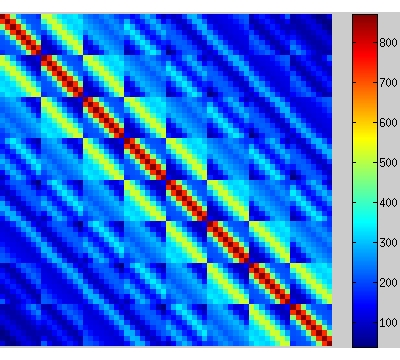
\includegraphics[width=\textwidth]{figures/ada}
    \caption{An example of $A^\dagger A$ for N=64 }
    \label{Figada}
  \end{center}
\end{figure}

\section{Implementation}
\label{s:implement}

\subsection{MATLAB Implementation}
\label{s:implement_matlab}

\paragraph{}
The algorithms as mentioned in Section 3.5 require computations 
of large matrices. In particular, they require eigenvalue computations, 
matrix-matrix multiplications, matrix-vector multiplications and other 
algebraic transformations. Considering MATLAB's capabilities to perform 
the required computations with programming abstractions, it is considered 
as an appropriate tool for initial implementations. Also, MATLAB's Toolbox 
for Image Processing provides additional advantage for exploratory analysis 
of images from Radio Interferometry data sets. 

\paragraph{}
Further, algorithmic implementations were developed for all four variants 
of Iterative Shrinkage Thresholding Algorithms. Exploratory analysis via 
empirical validation were carried out by investigating the run-time complexities 
of the algorithms. CPU time taken were recorded, compared and evaluated. 
Performance benchmark trials were carried out by varying the number 
of iterations and the penalty parameter for determining their optimal values. 
Objective function values at each iteration were stored with a specified
numerical accuracy. Robustness of the algorithmic implementation was validated
by performing repeated trials with varying data sets each representing 
single point source, double point sources and grid point sources.

\subsubsection{Input Data}

\paragraph{}
Initially, data sets with characteristics similar to the original data sets
of the FITS files were simulated using the AIPS tool for single point source 
and double point sources with varying fluxes. Each row of data set consist of
a $u,v,w$ co-ordinates, amplitude and phase of visibility measured. 

\subsubsection{Processing}

\paragraph{}Parameters required for processing the data sets are
\begin{itemize}
 \item Lipschitz constant ($L$) for fixed step size variants which is maximum
	eigenvalue of $A^\dagger A$.
 \item Backtracking parameter ($\eta$). For both backtracking variants $\eta$ value
       is taken as 1.125.
 \item Penalty parameter ($0 < \lambda < \infty$).
 \item Maximum Iteration Number ($maxiter$) which is one of the stopping criterion formats 
	the algorithms.
 \item Tolerance limit explained by equation (\ref{stopping}).
\end{itemize}

\paragraph{}
After parameters are decided, $A$ matrix is computed using $u-v$ co-ordinates from data sets
and regular $l-m$ grid using equation (\ref{Amat}). Visibilities are computed in $a+ib$ format
using phase and amplitude and were stored in $b$ vector which is our measurement vector.  
Further, each variants of algorithms require $A^ \dagger A$, $A^ \dagger b$ 
which are computed as discussed in Section 3.7. Finally, following processed inputs are
given to algorithms
\begin{itemize}
 \item $A^\dagger A$
 \item $A^\dagger b$
 \item Lipschitz constant ($L$) (for fixed step size)
 \item Penalty parameter ($\lambda$) 
 \item Backtracking Parameter ($\eta$) (for backtracking)
 \item Initial guess of solution which is zero vector
 \item Maximum iteration ($maxiter$)
 \item Tolerance limit (typically $10^{-7}$) 
\end{itemize}

\subsubsection{Output data}
\paragraph{}All four algorithms gives exactly the same solution vector with high numerical
accuracy for single point source and double point source data set. By plotting the objective 
function values with each iterations it was clear that FISTA variants perform better than 
ISTA. Further, backtracking algorithms scores over fixed step size algorithms for radio interferometric
data sets.

\subsection{C Implementation}
\label{s:implement_C}

\paragraph{}For the reasons of speed, efficiency, flexibility and to include 
Compressed Sensing formulation in GMRT pipeline, all algorithms are implemented in C.
Radio Interferometry data sets are available in Flexible Image Transport System 
(FITS) formats (see appendix). We use Read-Write FITS (RWFITS) \footnote{written by Prof.\ Jayaram N. Chengalur}.
for reading the FITS file, in a specific structure which is further read for 
$u,v,w$ and visibility data.

\paragraph{}The structure of C-code is shown in Figure (\ref{Figflow}). The Data, after being read 
from FITS file are given to processing block which compute the inputs needed by algorithms 
as discussed in previous section. Since there is lot of symmetry in $A^ \dagger A$ (discussed in Section 3.7)
 and $A$ (due to symmetry in $uv$ plane), there are options in the code for using these symmetries.
Finally these computed matrices are given to the Compressed Sensing solvers, each algorithm gives same solution image
with high precision accuracy. This reconstructed solution image is written back in to FITS file format using
cfitsio (see appendix) routines.

\paragraph{}For Basic linear algebra operations we have used intel's implementation of LAPACK and BLAS library,
which performs matrix-matrix, matrix-vector, eigenvalue computations efficiency.

\begin{figure}[!htbp]
  \begin{center}
      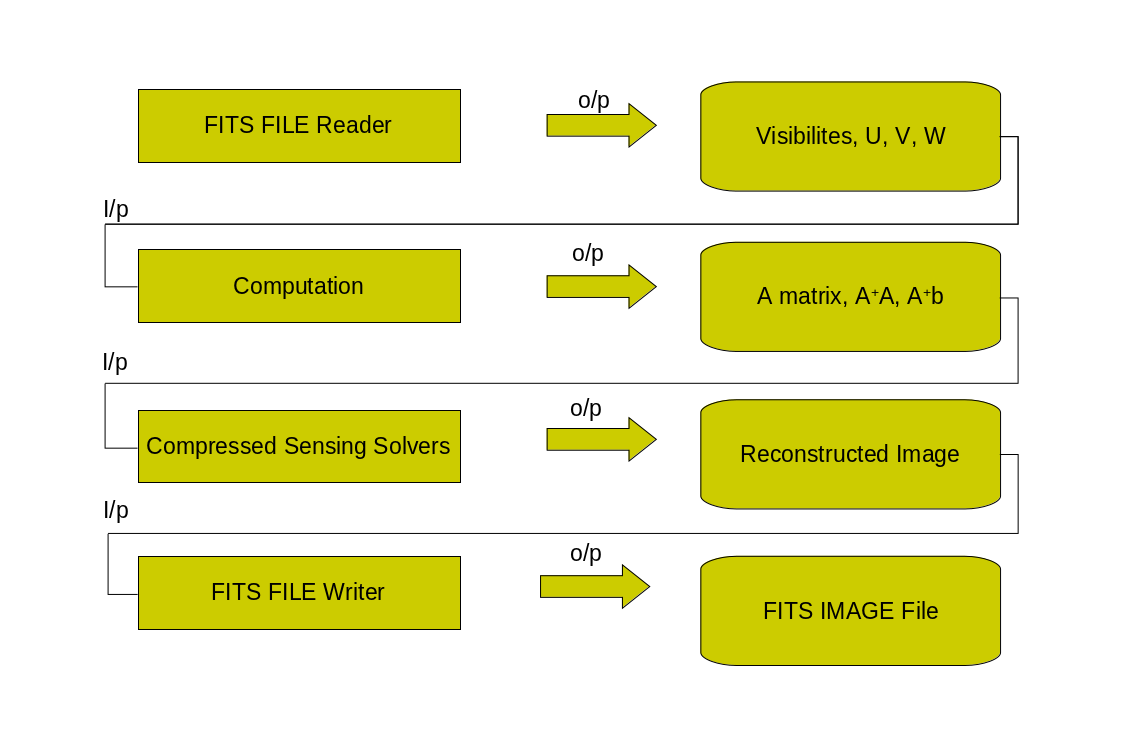
\includegraphics[width=6.1in,height=4in]{figures/flow}
    \caption{Flowchart of C Code}
    \label{Figflow}
  \end{center}
\end{figure}

 % methods
 \chapter{Results and Discussion}
\label{c:r_and_d}

\section{A Toy Model}
\label{s:toymodel}

\subsection{Formulation}
\label{s:toy_formalism}
\markboth{\MakeUppercase{\thechapter. Toy Models }}{\thechapter. Toy Models}

\paragraph{}To get the feel of Compressed Sensing, we applied its framework on various toy models. 
One such model is spike train model in which $A$ matrix or sensing matrix of order $M \times N$ is 
random Gaussian matrix with normalized i.i.d entries. We constructed hypothetical example with known $M=40$ 
random measurements ($b$ vector) for a particular $40 \times 100$ $A$ matrix and it is also known that $x$ 
vector which we have to reconstruct, has four spikes. Figure (\ref{Figorgvect} is an plot of original vector
in which $X$-axis denotes the component number and $Y$ axis represents values at each components. Indeed  
$x$ is sparse as most of its components are either zero or approximately equal to zero. We had also added 
normally distributed Gaussian noise in the measurement vector as in real scenario every measurements comes with the noise.


\subsection{Tools used}
\label{s:toy_tools}
\paragraph{}Next step was to apply compressed sensing or $\ell_1$ minimization algorithms to this problem, we used MATLAB 
as a tool for this analysis and CVX, which is matlab program for disciplined convex programming, is used to solve \ref{1.6}
formulated for this problem. ( for more information refer CVX user Guide ).

\subsection{Results and Discussion}
\label{s:toy_results}
\paragraph{}Figure \ref{Figorgvect} shows plot of original vector with X-axis as component number and 
Y-axis as corresponding value at each components. Figure shows that plotted vector is sparse and has 
only four significant values or spikes. 
\paragraph{}Figure \ref{Figrecvect} shows plot of reconstructed vector (shown with dotted red line) and
original vector (dotted blue line). With small variation reconstructed vector overlaps the original
vector.
\paragraph{}CVX internally use Interior point methods (\cite{karmarkar}) for solving equation (\ref{1.6}) for the given problem.
This basic linear programming method has no performance issues while dealing with problems of such small scale
but suffer for poor convergence rate otherwise. For this toy problem, interior point algorithm or CVX converges in 
127 iterations. Further, CVX does not require any penalty parameter for minimization process. 

\begin{figure}[!htbp]
  \begin{center}
      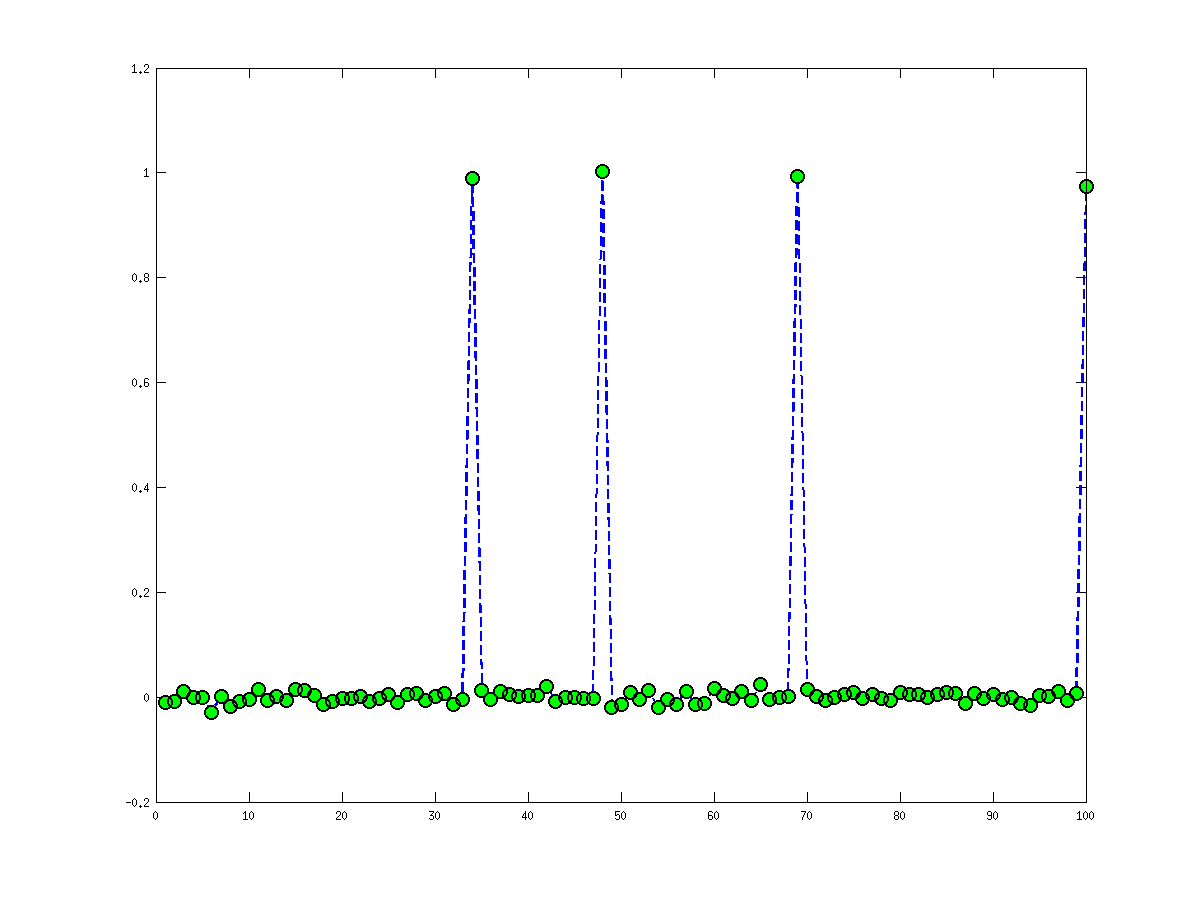
\includegraphics[width=6.1in,height=4in]{figures/orgvect}
    \caption{Original Vector}
    \label{Figorgvect}
  \end{center}

\end{figure}
\begin{figure}[!htbp]
  \begin{center}
      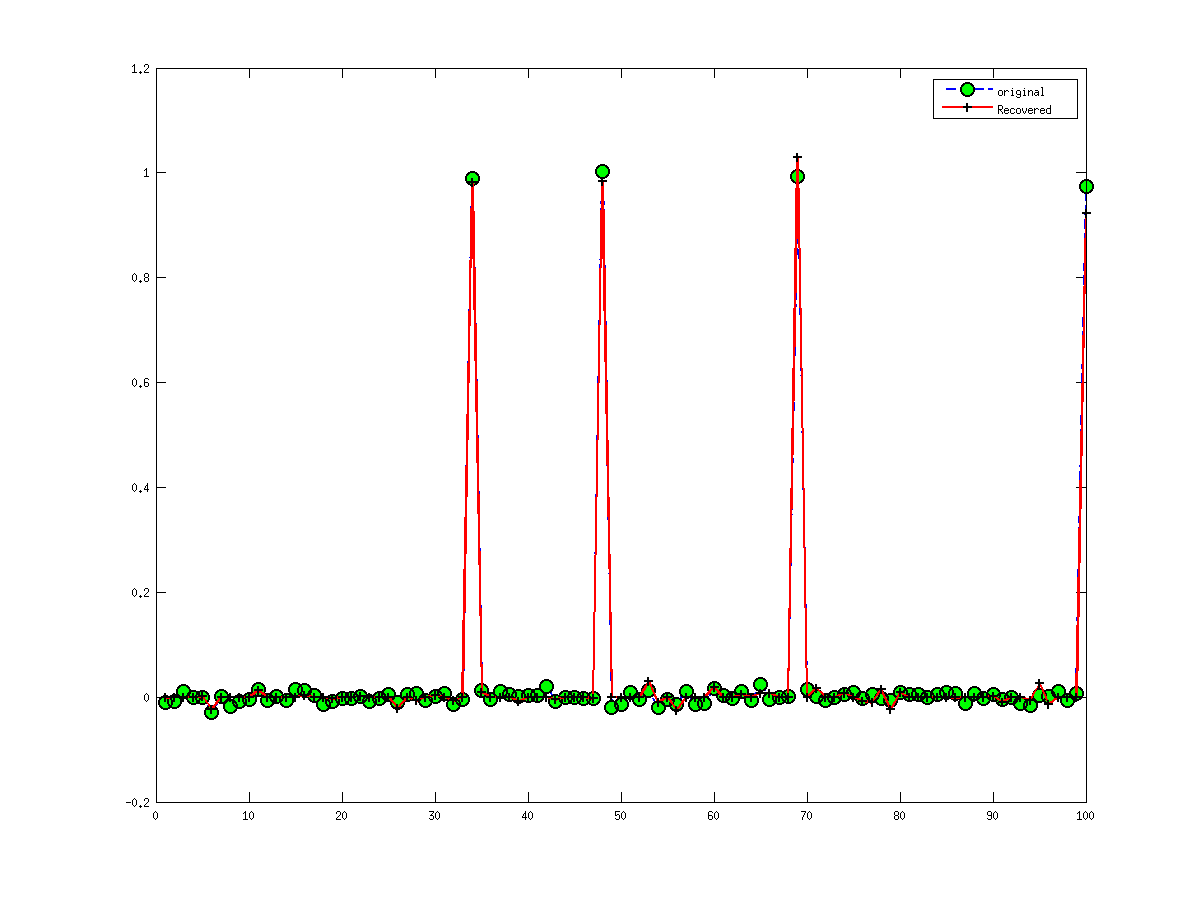
\includegraphics[width=6.1in,height=4in]{figures/recvect}
    \caption{Reconstructed Vector}
    \label{Figrecvect}
  \end{center}
\end{figure}

\section{Reconstructing Single and Double Point Sources}
\label{s:results_main}

\subsection{Input}
\label{s:results_input}
\paragraph{}We have considered the images of single point source with illumination 
at center pixel of the image and double point sources with at centre
and along the main diagonal. Both point sources have different fluxes and 
ratio of the fluxes at center to other is 0.8. We have used following input parameters
for the algorithms. 

\subsection{Input Parameters}
\label{s:results_input_p}
\paragraph{} Following are the input parameters used for reconstruction. 
\begin{itemize}
 \item Lipschitz constant ($L$) (for fixed step size variants) = maximum eigenvalue of $A^\dagger A$.
 \item Backtracking parameter ($\eta$) = 1.125.
 \item Varied Penalty parameter from ($10^{-4} < \lambda < 10^4$).
 \item Maximum Iteration Number ($maxiter$) = 10000.
 \item Tolerance limit = $10^{-7}$.
\end{itemize}

\subsection{Output}
\label{s:results_output}

\paragraph{}Figure \ref{Figsps} with $\lambda=1150$ shows reconstructed image of single point source of flux 0.4 at the center.
We had produced such images for various values of $\lambda$ to check the effect of $\lambda$ on
reconstruction. 

\paragraph{}Figure \ref{Figdps} with $\lambda=1150$ shows reconstructed image of double point source at specific
pixels. Recovered image has to ratio of fluxes (flux at center pixel : flux at other) is $\sim$ 0.8.

\begin{figure}[!htbp]
  \begin{center}
      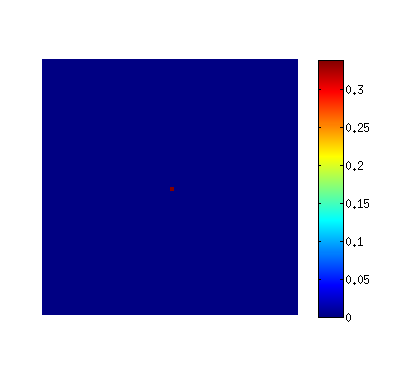
\includegraphics[width=5in,height=4in]{figures/sps}
    \caption{Reconstructed Image of Single point source with $\lambda$ = 1150}
    \label{Figsps}
  \end{center}
\end{figure}

\begin{figure}[!htbp]
  \begin{center}
      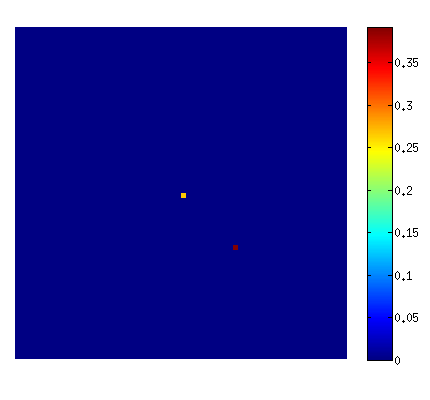
\includegraphics[width=5in,height=4in]{figures/dps}
    \caption{Reconstructed Image of Double point source with $\lambda$ = 1150}
    \label{Figdps}
  \end{center}
\end{figure}

\paragraph{}Figure \ref{Figsubplot} shows the reconstructed image with different
$\lambda$ values for all solvers. $Fista_F$ denotes Fista with fixed step size and 
similarly others.

\begin{figure}[!htbp]
  \begin{center}
      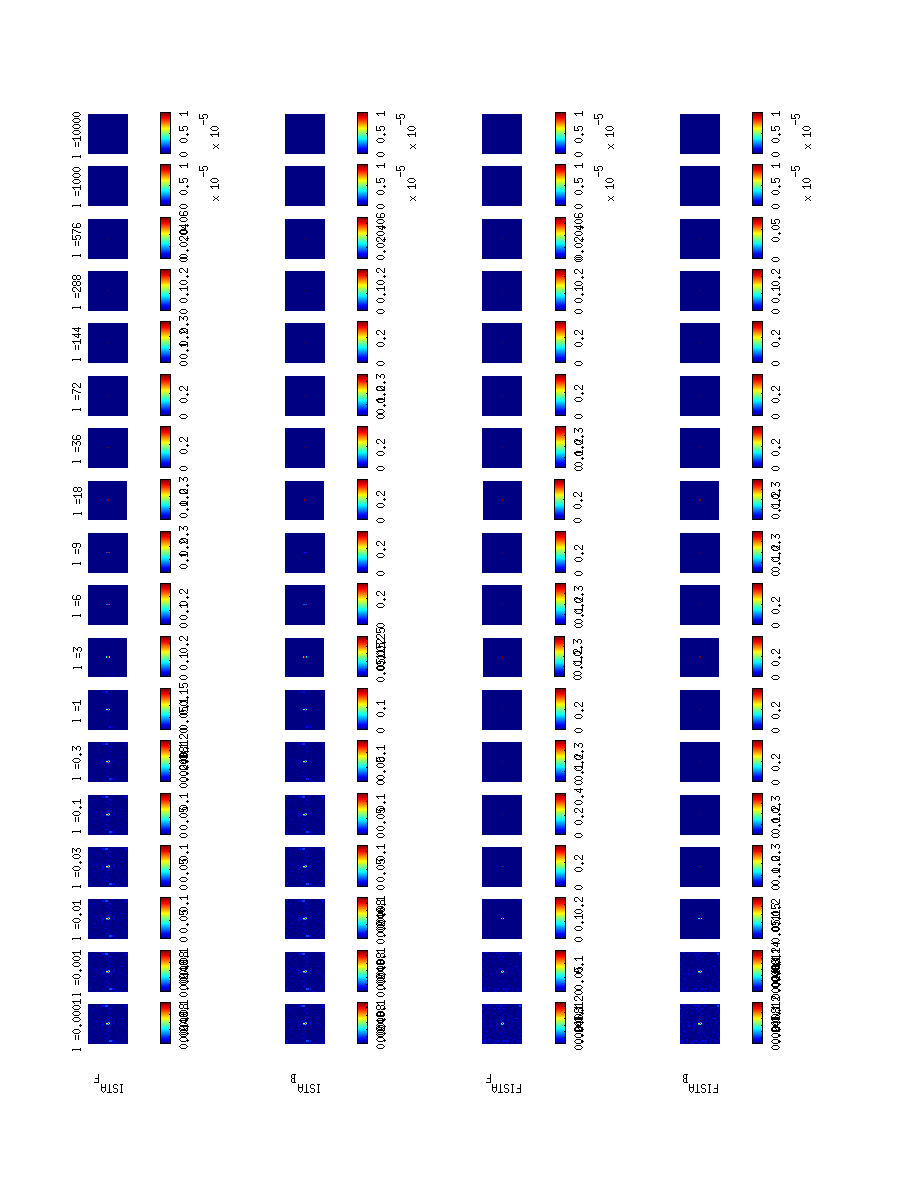
\includegraphics[width=7in,height=8in]{figures/subplots}
    \caption{Reconstructed Image of Double point source with $\lambda$ = 1150}
    \label{Figsubplot}
  \end{center}
\end{figure}

\section{Discussion}
\label{s:discussion}

\subsection{Effect of Penalty Parameter}
\label{s:discussion_pp}

\paragraph{}Equation (\ref{1.6}) in which residuals are measured with $\ell_2$ norm and regularization is 
done with $\ell_1$ norm, seeks the solution that is close (in $\ell_2$ norm) to the 
measured corrupted signal $b$ and the one that is sparse. By varying the penalty parameter $\lambda$
( aka regularization parameter) one can find out the optimal trade-off between $\parallel Ax-b \parallel_{\ell_2}$
(fidelity term)and $\parallel x \parallel_{\ell_1}$( sparsity inducing term ).
\paragraph{}Penalty parameter varies form 0 to $\infty$. In practical applications, for smaller value of $\lambda$ in 
 equation (\ref{1.6}) put more emphasis on fidelity term, thereby neglecting sparsity in the solution. On the other
hand, larger values of $ \lambda$ put more weight on sparsity inducing term and leads to
sparsest solution which is zero vector. So finding out the optimal trade-off between these bi-criterion objectives requires
optimal value of regularization parameter.
\paragraph{}Figure \ref{Figsmalllam} shows the reconstructed image of single point source with point source 
at the center. Due to very small $\lambda=10^{-4}$, this leads to just the least solution which is not sparse.
\paragraph{}Figure \ref{Figlargelam} shows the reconstructed image of same single point source with point source 
at the center. Large value $\lambda=10^{4}$ gives zero solution as discussed.
\paragraph{}For certain optimal $\lambda = 1150$ (found out by simulations), Figure  shows reconstruction
of single point source exactly.

\begin{figure}[!htbp]
  \begin{center}
      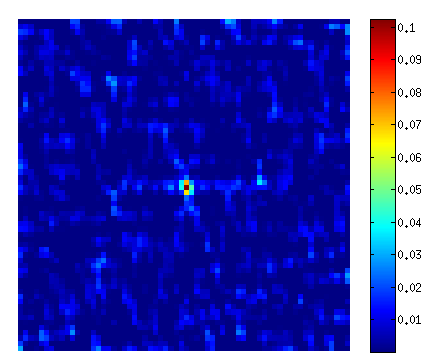
\includegraphics[width=4in,height=3in]{figures/spsn}
    \caption{Reconstruction of single point source for $\lambda = 0.001$}
    \label{Figsmalllam}
  \end{center}
\end{figure}

\begin{figure}[!htbp]
  \begin{center}
      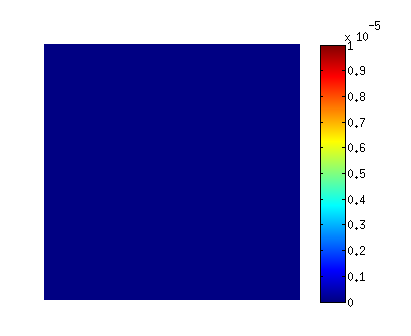
\includegraphics[width=5in,height=4in]{figures/spss}
    \caption{Reconstruction of single point source  for $\lambda = 10000$}
    \label{Figlargelam}
  \end{center}
\end{figure}

\newpage
\subsection{Convergence of algorithms}
\label{s:discussion_convergence}

\begin{figure}[!htbp]
  \begin{center}
      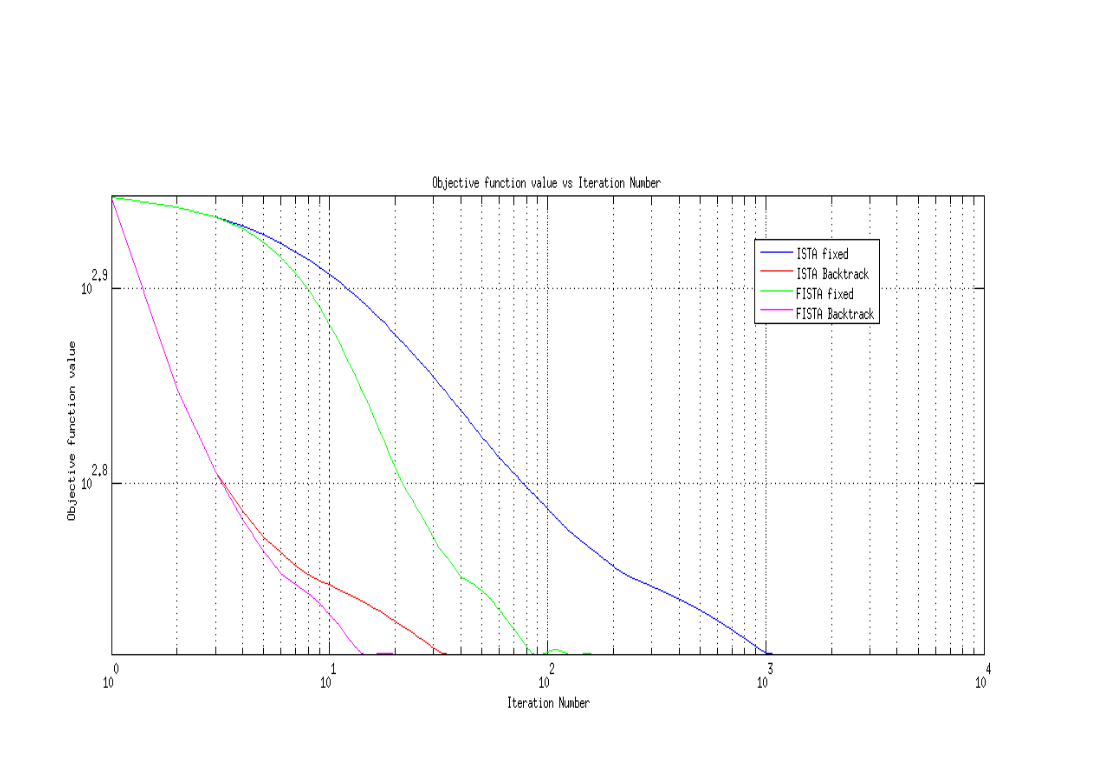
\includegraphics[width=6.1in,height=4in]{figures/convergence}
    \caption{Convergence of Algorithms}
    \label{Figconvergence}
  \end{center}
\end{figure}

\paragraph{}Figure \ref{Figconvergence}, shows the convergence of algorithms with 
respect to iteration number. It is clear that FISTA shows better performance 
than ISTA algorithms which is also theoretically proved. Further backtracking variants of both algorithms seems to 
perform much better then their corresponding fixed step size variants. All
four algorithms reaches the same optimal value and with same reconstructed image.

\newpage
\subsection{Flux fidelity}
\label{s:discussion_ff}

\paragraph{}Single point source and double point source reconstruction discussed in last chapter
are done with varying fluxes of illuminated pixels of image. This is done to check flux fidelity
with the penalty parameter. We have used various data set for single point source of fluxes 0.05, 0.1,
0.5, 1, 10 and 100 and double point sources we have used flux ratios as 0.1, 0.2, 0.4, 0.6 and 0.8.
\ref{Figflux} shows one of the result for single point source of flux 0.4.

\paragraph{}Figure \ref{Figflux} shows the plot peak value of the reconstructed image of 
single point source with flux value 0.4 (discussed in Section 6.3) with respect to penalty parameter varying from $10^-4$
to $10^4$ (Reconstructed Images in this range of penalty parameter can be seen in Fig 6.3 in 
Chapter 6). It is clear from the plot that certain optimal range of penalty parameter flux of 
single point source recovered is 0.4. 


\begin{figure}[!htbp]
  \begin{center}
      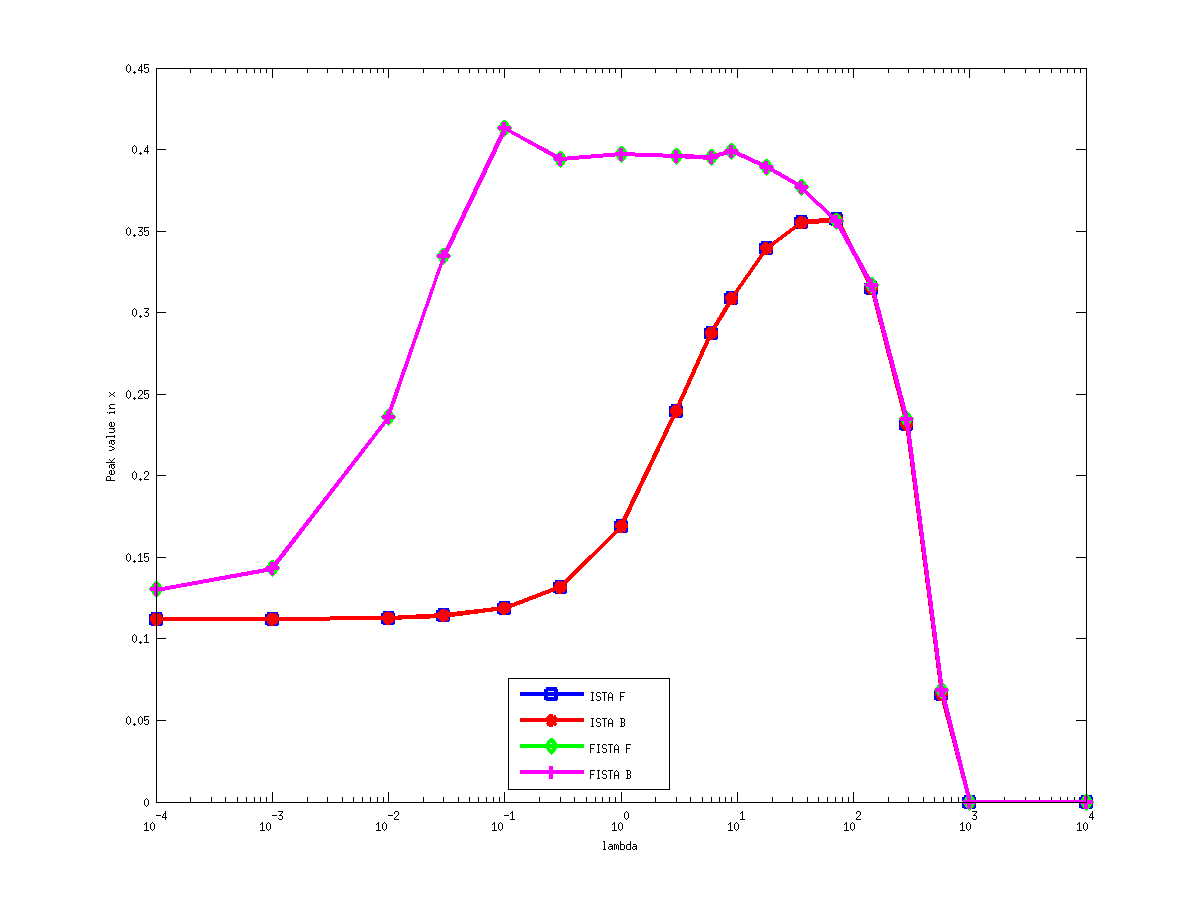
\includegraphics[width=6.1in,height=4in]{figures/pv}
    \caption{Peak Value vs Penalty Parameter}
    \label{Figflux}
  \end{center}
\end{figure}

 % results and discussion
 \chapter{Summary and Conclusion}
\label{c:conclusion}

We have evaluated a new frame work called Compressed Sensing for image reconstruction
problem in Radio Interferometry. We have explored the class of algorithms
called Proximal Gradient methods for efficient algorithms suitable
for Radio-interferometric data. Finally we concluded that ISTA and FISTA
algorithms along with their variants gives better performance and shows significant improvement 
in image visual quality over mainstream deconvolution algorithms like CLEAN. 
Further analysis, and work by other authors show that FISTA and its 
variants are capable of competing favourably with traditional image reconstruction methods 
in radio astronomy in normal scenarios, and will do much better in special cases (like 3D imaging,
multi-frequency synthesis etc). We have, though a toy model, investigated and identified the core
problems involved in such an exercise, and have gone on to implement a working code for applying compressed
sensing to radio interferometric data from the GMRT. Along with collaborators at NCRA, we are
currently involved in solving the remaining outstanding issues - namely, choosing an optimal penalty parameter,
fidelity of flux reconstruction, and computational efficiency for large data sets. The code, which is a result
of this project, will be further developed at NCRA into a full-fledged pipeline for the GMRT data, over the coming
months. Possibilities for future work include the following:
\begin{enumerate}

\item  To estimate optimal value of penalty parameter
\item  To solve full Van Cittert–Zernike equation.
\item  To create a library of basis matrix.
\item  Modify the algorithm for gridded Visibilities.
\item  Modify the C code for all the above cases.

\end{enumerate}
 % summary, conclusion, future work

 \bibliographystyle{abbrv} % some standard bibtex style
 \bibliography{report}     % should be in the .bib format
 \addcontentsline{toc}{chapter}{Bibliography}

 % any additional material that belongs to appendices
 % \appendix
 % \input{appendix1}
 % \input{appendix2}
\end{document}
